\documentclass[11pt,a4paper]{book}%

\usepackage{titlesec} 

% \usepackage[compact,explicit]{titlesec}

\usepackage[basque]{babel}

\addto\captionsbasque{
  \renewcommand{\contentsname}%
    {Gaien aurkibidea}%
}


%\newcommand{\periodafter}[1]{#1.}

%\titleformat{\section}%
%{\large\bfseries}
%{\thesection\periodafter}{1em}{}

%\titleformat{\subsection}%
%{\bfseries}
%{\thesection.\thesubsection\periodafter}{1em}{}

%\titleformat{\subsubsection}%
%{\bfseries}
%{\thesection.\thesubsection.\thesubsubsection\periodafter}{1em}{}


% SOURCE:
% https://tex.stackexchange.com/questions/595713/fancyhdrs-extra-dot-in-header-for-section-title-how-to-remove
%\titleformat{\section}{\large\bfseries}{}{0pt}{\thesection .\quad #1} % section number with dot
%\titleformat{\subsection}{\bfseries}{}{0pt}{\thesubsection .\quad #1} % subsection number with dot  

%\titleformat{\chapter}[block]
%{\Large\bfseries}{\thechapter}{12pt}{#1}

% \titlelabel{\thetitle.\quad}

% \renewcommand\thechapter{\arabic{chapter}}


% *********************************** TOC
\usepackage{tocloft} % added to correct TOC%
\renewcommand{\cftchapaftersnum}{.}% Add dot after chap number in ToC
\renewcommand{\cftsecaftersnum}{.}% Add dot after section number in ToC
\renewcommand{\cftsubsecaftersnum}{.}% Add dot after subsection number in ToC
% *********************************** TOC


%% chapter header
\addto\captionsbasque{\renewcommand{\chaptername}{
%Kapitulu
}}

\addto\captionsbasque{
\renewcommand{\chapterautorefname}{kapitulua}
}

% \titleformat{\chapter}{\LARGE\bfseries}{\thechapter.\ }{0em}{}

\titleformat{\chapter}[display]
   {\bfseries\Large}
   {\filright\MakeUppercase{\chaptertitlename} %\Huge
   }
   {1ex}
   %{\titlerule\vspace{1ex}\ifnum\value{chapter}>0\relax\thechapter.\hspace{1.5 mm}\MakeUppercase{#1} \filleft\fi}
   {\titlerule\vspace{1ex}\ifnum\value{chapter}>0\relax\thechapter.\hspace{1.5 mm} \filleft\fi}  
   % {\titlerule\vspace{1ex}\filleft}
   [\vspace{1ex}\titlerule]
  
% no page number on chapter page
\makeatletter
\let\ps@plain\ps@empty
\makeatother

\usepackage[dvipsnames,usenames]{xcolor}

\definecolor{editorGray}{rgb}{0.95, 0.95, 0.95}
\definecolor{editorOcher}{rgb}{1, 0.5, 0} % #FF7F00 -> rgb(239, 169, 0)
\definecolor{editorGreen}{rgb}{0, 0.5, 0} % #007C00 -> rgb(0, 124, 0)
    
\usepackage{soul}
\usepackage{hyperref}
\hypersetup{colorlinks=true,linkcolor=blue, linktocpage}
\usepackage{menukeys}
% \usepackage{mdframed}
\usepackage{amsmath}
\usepackage[T1]{fontenc}
\usepackage{amsfonts}
\usepackage[utf8x]{inputenc}


% Source: https://www.overleaf.com/learn/latex/Headers_and_footers
\usepackage{fancyhdr}
\pagestyle{fancy}
% Source: https://tex.stackexchange.com/questions/228362/get-sectionmark-in-fancyhdr-without-chapter-number
% https://en.wikibooks.org/wiki/LaTeX/Customizing_Page_Headers_and_Footers
% Note that these redefinitions must be inserted after the first call of \pagestyle{fancy}.
\renewcommand{\chaptermark}[1]{\markboth{#1}{}}
\fancyhf{}
\fancyhead[LE,RO]{\thepage}
\fancyhead[RE]{HTML5 lengoaia eta JavaScript APIak}
% http://tug.ctan.org/tex-archive/macros/latex/contrib/fancyhdr/fancyhdr.pdf \nouppercase is needed for making uppercase index header
\fancyhead[LO]{\nouppercase{\leftmark}}

\usepackage[tikz]{bclogo}
\usepackage{comment}
\usepackage{graphicx}
\usepackage[a4paper,paperwidth=17.0cm,paperheight=24cm, top=2.5cm, bottom=2.5cm, left=2.2cm, right=2.2cm]%
{geometry}

\usepackage{wrapfig}

\usepackage{fontawesome}

% ALERT INFO BOX
% \usepackage{xcolor}
\definecolor{infobackground}{RGB}{217,237,247}
\definecolor{infoforeground}{RGB}{58,135,173}
\definecolor{infoborder}{RGB}{188,232,241}

\usepackage{environ}
\usetikzlibrary{fit,backgrounds,calc}

\NewEnviron{alertinfo}[1]
{
    \begin{tikzpicture}
    \node[inner sep=0pt,
          draw=infoborder,
          line width=1.2pt,
          fill=infobackground] (box) {\parbox[t]{.95\textwidth}
        {%
            \begin{minipage}{.15\textwidth}
                \centering\tikz[scale=3]
                \node[scale=1]
                {
                    \includegraphics[scale=0.15]{img/alertinfo.png}
                };
            \end{minipage}%
           \begin{minipage}{.75\textwidth}
                \vskip 10pt
                \textbf{\textcolor{infoforeground}{#1}}\par\smallskip
                \textcolor{infoforeground}{\BODY}
                \par\smallskip
            \end{minipage}\hfill
        }%
    };

    \end{tikzpicture}
}

\usepackage{adjustbox}
% END ALERT INFO BOX


%\usepackage{geometry}
\usepackage{marginnote}

\usepackage{times}
\usepackage{listings}
\usepackage{textcomp}

\definecolor{lightgray}{rgb}{.9,.9,.9}
\definecolor{darkgray}{rgb}{.4,.4,.4}
\definecolor{purple}{rgb}{0.65, 0.12, 0.82}


\lstdefinelanguage{JavaScript}{
  keywords={break, case, catch, const, continue, debugger, default, delete, do, else, false, finally, for, function, if, in, instanceof, let, new, null, return, switch, this, throw, true, try, typeof, var, void, while, with, forEach},
  morecomment=[l]{//},
  morecomment=[s]{/*}{*/},
  morestring=[b]',
  morestring=[b]",
  ndkeywords={class, export, boolean, throw, implements, import, this},
  keywordstyle=\color{blue}\bfseries,
  ndkeywordstyle=\color{darkgray}\bfseries,
  identifierstyle=\color{black},
  commentstyle=\color{purple}\ttfamily,
  stringstyle=\color{red}\ttfamily,
  sensitive=true
}

\lstset{
   language=JavaScript,
   backgroundcolor=\color{white},
   extendedchars=true,
   basicstyle=\footnotesize\ttfamily,
   showstringspaces=false,
   showspaces=false,
   numbers=left,
   numberstyle=\footnotesize,
   numbersep=9pt,
   tabsize=2,
   breaklines=true,
   showtabs=false,
   captionpos=b,
   upquote=true,
   literate={á}{{\'a}}1 {ã}{{\~a}}1 {é}{{\'e}}1 {í}{{\'i}}1 {ó}{{\'o}}1 {ú}{{\'u}}1,
}

 \lstdefinelanguage{JavaScript}{
      morekeywords={break, case, catch, const, continue, debugger, default, delete,         do, else, false, finally, for, function, if, in, instanceof, let, new, null, return, switch, this, throw, true, try, typeof, var, void, while, with},
      morecomment=[s]{/*}{*/},
      morecomment=[l]//,
      morestring=[b]",
      morestring=[b]'
    }
    \lstdefinelanguage{CSS}{
      keywords={accelerator,azimuth,background,background-attachment,
            background-color,background-image,background-position,
            background-position-x,background-position-y,background-repeat,
            behavior,border,border-bottom,border-bottom-color,
            border-bottom-style,border-bottom-width,border-collapse,
            border-color,border-left,border-left-color,border-left-style,
            border-left-width,border-right,border-right-color,
            border-right-style,border-right-width,border-spacing,
            border-style,border-top,border-top-color,border-top-style,
            border-top-width,border-width,bottom,caption-side,clear,
            clip,color,content,counter-increment,counter-reset,cue,
            cue-after,cue-before,cursor,direction,display,elevation,
            empty-cells,filter,float,font,font-family,font-size,
            font-size-adjust,font-stretch,font-style,font-variant,
            font-weight,height,ime-mode,include-source,
            layer-background-color,layer-background-image,layout-flow,
            layout-grid,layout-grid-char,layout-grid-char-spacing,
            layout-grid-line,layout-grid-mode,layout-grid-type,left,
            letter-spacing,line-break,line-height,list-style,
            list-style-image,list-style-position,list-style-type,margin,
            margin-bottom,margin-left,margin-right,margin-top,
            marker-offset,marks,max-height,max-width,min-height,
            min-width,-moz-binding,-moz-border-radius,
            -moz-border-radius-topleft,-moz-border-radius-topright,
            -moz-border-radius-bottomright,-moz-border-radius-bottomleft,
            -moz-border-top-colors,-moz-border-right-colors,
            -moz-border-bottom-colors,-moz-border-left-colors,-moz-opacity,
            -moz-outline,-moz-outline-color,-moz-outline-style,
            -moz-outline-width,-moz-user-focus,-moz-user-input,
            -moz-user-modify,-moz-user-select,orphans,outline,
            outline-color,outline-style,outline-width,overflow,
            overflow-X,overflow-Y,padding,padding-bottom,padding-left,
            padding-right,padding-top,page,page-break-after,
            page-break-before,page-break-inside,pause,pause-after,
            pause-before,pitch,pitch-range,play-during,position,quotes,
            -replace,richness,right,ruby-align,ruby-overhang,
            ruby-position,-set-link-source,size,speak,speak-header,
            speak-numeral,speak-punctuation,speech-rate,stress,
            scrollbar-arrow-color,scrollbar-base-color,
            scrollbar-dark-shadow-color,scrollbar-face-color,
            scrollbar-highlight-color,scrollbar-shadow-color,
            scrollbar-3d-light-color,scrollbar-track-color,table-layout,
            text-align,text-align-last,text-decoration,text-indent,
            text-justify,text-overflow,text-shadow,text-transform,
            text-autospace,text-kashida-space,text-underline-position,top,
            unicode-bidi,-use-link-source,vertical-align,visibility,
            voice-family,volume,white-space,widows,width,word-break,
            word-spacing,word-wrap,writing-mode,z-index,zoom},  
      sensitive=true,
      morecomment=[l]{//},
      morecomment=[s]{/*}{*/},
      morestring=[b]',
      morestring=[b]",
      alsoletter={:},
      alsodigit={-}
    }
    \lstdefinelanguage{HTML5}{
            language=html,
            sensitive=true, 
            alsoletter={<>=-},
            otherkeywords={
            % HTML tags
            <, </, >,
            </a, <a, </a>,
            </abbr, <abbr, </abbr>,
            </address, <address, </address>,
            </area, <area, </area>,
            </area, <area, </area>,
            </article, <article, </article>,
            </aside, <aside, </aside>,
            </audio, <audio, </audio>,
            </audio, <audio, </audio>,
            </b, <b, </b>,
            </base, <base, </base>,
            </bdi, <bdi, </bdi>,
            </bdo, <bdo, </bdo>,
            </blockquote, <blockquote, </blockquote>,
            </body, <body, </body>,
            </br, <br, </br>,
            </button, <button, </button>,
            </canvas, <canvas, </canvas>,
            </caption, <caption, </caption>,
            </cite, <cite, </cite>,
            </code, <code, </code>,
            </col, <col, </col>,
            </colgroup, <colgroup, </colgroup>,
            </data, <data, </data>,
            </datalist, <datalist, </datalist>,
            </dd, <dd, </dd>,
            </del, <del, </del>,
            </details, <details, </details>,
            </dfn, <dfn, </dfn>,
            </div, <div, </div>,
            </dl, <dl, </dl>,
            </dt, <dt, </dt>,
            </em, <em, </em>,
            </embed, <embed, </embed>,
            </fieldset, <fieldset, </fieldset>,
            </figcaption, <figcaption, </figcaption>,
            </figure, <figure, </figure>,
            </footer, <footer, </footer>,
            </form, <form, </form>,
            </h1, <h1, </h1>,
            </h2, <h2, </h2>,
            </h3, <h3, </h3>,
            </h4, <h4, </h4>,
            </h5, <h5, </h5>,
            </h6, <h6, </h6>,
            </head, <head, </head>,
            </header, <header, </header>,
            </hr, <hr, </hr>,
            </html, <html, </html>,
            </i, <i, </i>,
            </iframe, <iframe, </iframe>,
            </img, <img, </img>,
            </input, <input, </input>,
            </ins, <ins, </ins>,
            </kbd, <kbd, </kbd>,
            </keygen, <keygen, </keygen>,
            </label, <label, </label>,
            </legend, <legend, </legend>,
            </li, <li, </li>,
            </link, <link, </link>,
            </main, <main, </main>,
            </map, <map, </map>,
            </mark, <mark, </mark>,
            </math, <math, </math>,
            </menu, <menu, </menu>,
            </menuitem, <menuitem, </menuitem>,
            </meta, <meta, </meta>,
            </meter, <meter, </meter>,
            </nav, <nav, </nav>,
            </noscript, <noscript, </noscript>,
            </object, <object, </object>,
            </ol, <ol, </ol>,
            </optgroup, <optgroup, </optgroup>,
            </option, <option, </option>,
            </output, <output, </output>,
            </p, <p, </p>,
            </param, <param, </param>,
            </pre, <pre, </pre>,
            </progress, <progress, </progress>,
            </q, <q, </q>,
            </rp, <rp, </rp>,
            </rt, <rt, </rt>,
            </ruby, <ruby, </ruby>,
            </s, <s, </s>,
            </samp, <samp, </samp>,
            </script, <script, </script>,
            </section, <section, </section>,
            </select, <select, </select>,
            </small, <small, </small>,
            </source, <source, </source>,
            </span, <span, </span>,
            </strong, <strong, </strong>,
            </style, <style, </style>,
            </summary, <summary, </summary>,
            </sup, <sup, </sup>,
            </svg, <svg, </svg>,
            </table, <table, </table>,
            </tbody, <tbody, </tbody>,
            </td, <td, </td>,
            </template, <template, </template>,
            </textarea, <textarea, </textarea>,
            </tfoot, <tfoot, </tfoot>,
            </th, <th, </th>,
            </thead, <thead, </thead>,
            </time, <time, </time>,
            </title, <title, </title>,
            </tr, <tr, </tr>,
            </track, <track, </track>,
            </u, <u, </u>,
            </ul, <ul, </ul>,
            </var, <var, </var>,
            </video, <video, </video>,
            </wbr, <wbr, </wbr>,
            />%, <!
            },  
            ndkeywords={
            % General
            =,
            % HTML attributes
            accept=, accept-charset=, accesskey=, action=, align=, alt=, async=, autocomplete=, autofocus=, autoplay=, autosave=, bgcolor=, border=, buffered=, challenge=, charset=, checked=, cite=, class=, code=, codebase=, color=, cols=, colspan=, content=, contenteditable=, contextmenu=, controls=, coords=, data=, datetime=, default=, defer=, dir=, dirname=, disabled=, download=, draggable=, dropzone=, enctype=, for=, form=, formaction=, headers=, height=, hidden=, high=, href=, hreflang=, http-equiv=, icon=, id=, ismap=, itemprop=, keytype=, kind=, label=, lang=, language=, list=, loop=, low=, manifest=, max=, maxlength=, media=, method=, min=, multiple=, name=, novalidate=, open=, optimum=, pattern=, ping=, placeholder=, poster=, preload=, pubdate=, radiogroup=, readonly=, rel=, required=, reversed=, rows=, rowspan=, sandbox=, scope=, scoped=, seamless=, selected=, shape=, size=, sizes=, span=, spellcheck=, src=, srcdoc=, srclang=, start=, step=, style=, summary=, tabindex=, target=, title=, type=, usemap=, value=, width=, wrap=,
            % CSS properties
            accelerator:,azimuth:,background:,background-attachment:,
            background-color:,background-image:,background-position:,
            background-position-x:,background-position-y:,background-repeat:,
            behavior:,border:,border-bottom:,border-bottom-color:,
            border-bottom-style:,border-bottom-width:,border-collapse:,
            border-color:,border-left:,border-left-color:,border-left-style:,
            border-left-width:,border-right:,border-right-color:,
            border-right-style:,border-right-width:,border-spacing:,
            border-style:,border-top:,border-top-color:,border-top-style:,
            border-top-width:,border-width:,bottom:,caption-side:,clear:,
            clip:,color:,content:,counter-increment:,counter-reset:,cue:,
            cue-after:,cue-before:,cursor:,direction:,display:,elevation:,
            empty-cells:,filter:,float:,font:,font-family:,font-size:,
            font-size-adjust:,font-stretch:,font-style:,font-variant:,
            font-weight:,height:,ime-mode:,include-source:,
            layer-background-color:,layer-background-image:,layout-flow:,
            layout-grid:,layout-grid-char:,layout-grid-char-spacing:,
            layout-grid-line:,layout-grid-mode:,layout-grid-type:,left:,
            letter-spacing:,line-break:,line-height:,list-style:,
            list-style-image:,list-style-position:,list-style-type:,margin:,
            margin-bottom:,margin-left:,margin-right:,margin-top:,
            marker-offset:,marks:,max-height:,max-width:,min-height:,
            min-width:,transition-duration:,transition-property:,
            transition-timing-function:,transform:,
            -moz-transform:,-moz-binding:,-moz-border-radius:,
            -moz-border-radius-topleft:,-moz-border-radius-topright:,
            -moz-border-radius-bottomright:,-moz-border-radius-bottomleft:,
            -moz-border-top-colors:,-moz-border-right-colors:,
            -moz-border-bottom-colors:,-moz-border-left-colors:,-moz-opacity:,
            -moz-outline:,-moz-outline-color:,-moz-outline-style:,
            -moz-outline-width:,-moz-user-focus:,-moz-user-input:,
            -moz-user-modify:,-moz-user-select:,orphans:,outline:,
            outline-color:,outline-style:,outline-width:,overflow:,
            overflow-X:,overflow-Y:,padding:,padding-bottom:,padding-left:,
            padding-right:,padding-top:,page:,page-break-after:,
            page-break-before:,page-break-inside:,pause:,pause-after:,
            pause-before:,pitch:,pitch-range:,play-during:,position:,quotes:,
            -replace:,richness:,right:,ruby-align:,ruby-overhang:,
            ruby-position:,-set-link-source:,size:,speak:,speak-header:,
            speak-numeral:,speak-punctuation:,speech-rate:,stress:,
            scrollbar-arrow-color:,scrollbar-base-color:,
            scrollbar-dark-shadow-color:,scrollbar-face-color:,
            scrollbar-highlight-color:,scrollbar-shadow-color:,
            scrollbar-3d-light-color:,scrollbar-track-color:,table-layout:,
            text-align:,text-align-last:,text-decoration:,text-indent:,
            text-justify:,text-overflow:,text-shadow:,text-transform:,
            text-autospace:,text-kashida-space:,text-underline-position:,top:,
            unicode-bidi:,-use-link-source:,vertical-align:,visibility:,
            voice-family:,volume:,white-space:,widows:,width:,word-break:,
            word-spacing:,word-wrap:,writing-mode:,z-index:,zoom:
            },  
            morecomment=[s]{<!--}{-->},
            tag=[s]
    }

    \lstset{%
        % Basic design
        backgroundcolor=\color{editorGray},
        basicstyle={\small\ttfamily},   
        frame=l,
        numbers=left,
        stepnumber=1,
        firstnumber=1,
        numberfirstline=true,
        % Code design   
        keywordstyle=\color{blue}\bfseries,
        commentstyle=\color{darkgray}\ttfamily,
        ndkeywordstyle=\color{editorGreen}\bfseries,
        stringstyle=\color{editorOcher},
        % Code
        language=HTML5,
        alsodigit={.:;},
        tabsize=2,
        showtabs=false,
        showspaces=false,
        showstringspaces=false,
        extendedchars=true,
    }
    
   % \lstset{prebreak=\raisebox{0ex}[0ex][0ex]
    %    {\ensuremath{\hookrightarrow}}}
\lstset{postbreak=\raisebox{0ex}[0ex][0ex]
        {\ensuremath{\hookrightarrow\space}}}
\lstset{breaklines=true, breakatwhitespace=true}

\sethlcolor{lightgray}

\newcommand{\hlc}[2][yellow]{ {\sethlcolor{#1} \hl{#2}} }


% \usepackage{jslistings} % colorize nodejs, js lstlisting 
\renewcommand{\lstlistingname}{Listatu }% Listing -> Algorithm

\usepackage{fancyvrb} % verbatim with font size

%\renewcommand{\thefootnote}{\arabic{footnote}}
% start sections with an integer (no decimals)

%\renewcommand{\thechapter}{\arabic{chapter}.}
%\renewcommand{\thesection}{\arabic{chapter}.\arabic{section}.{}}
%\renewcommand{\thesubsection}{\arabic{chapter}.\arabic{section}.\arabic{subsection}.{}}

%\renewcommand\thesection{\thechapter.\arabic{section}.}
%\renewcommand\thesubsection{\thesection\arabic{subsection}.}
%\renewcommand\thesubsubsection{\thesubsection\arabic{subsubsection}.}



% add dot after subsection
% Source: https://latex.org/forum/viewtopic.php?t=6404
%\makeatletter
%\g@addto@macro\thesubsection.
%\makeatother

%http://tex.stackexchange.com/questions/30720/footnote-without-a-marker
\newcommand\blfootnote[1]{%
  \begingroup
  \renewcommand\thefootnote{}\footnote{#1}%
  \addtocounter{footnote}{-1}%
  \endgroup
}

% https://tex.stackexchange.com/questions/17489/change-caption-name-of-figures
\addto\captionsbasque{\renewcommand{\figurename}{irudia}}
\addto\captionsbasque{\renewcommand{\tablename}{taula}}
\addto\captionsbasque{\renewcommand{\lstlistingname}{listatua}}

% https://tex.stackexchange.com/questions/331722/ordinal-captions-of-figures-with-basque-babel-in-tufte-book
\makeatletter
\addto\extrasbasque{%
  \def\fnum@figure{\thefigure.\nobreakspace\figurename}%
  \def\fnum@table{\thetable.\nobreakspace\tablename}%
  \def\fnum@lstlisting{\thelstlisting.\nobreakspace\lstlistingname}%
}
\makeatother


\usepackage{imakeidx}
\indexsetup{level=\chapter}
\makeindex 
% \usepackage{idxlayout}


\usepackage{booktabs}
\usepackage{pdfpages}

% https://tex.stackexchange.com/questions/31535/index-is-incorrectly-listed-in-the-table-of-contents
% \usepackage[nottoc,notbib]{tocbibind}

% Remove headers from empty pages https://tex.stackexchange.com/a/1684/69426
\usepackage{emptypage}

\begin{document}

% https://tex.stackexchange.com/questions/130440/how-to-change-the-name-of-index-section
\renewcommand\indexname{Kontzeptuen aurkibidea}


%Redefine the index environment
%\makeatletter
%\renewenvironment{theindex}{%
%    \renewcommand{\leftmark}{Index}
%    \chapter{Index}
%    \phantomsecion
%    \addcontentsline{toc}{chapter}{Index}
%    \vspace{1em}
%    \columnseprule \z@
%    \columnsep 35\p@
%    \idx@heading
%    \index@preamble\par\nobreak
%    \thispagestyle{\indexpagestyle}\parindent\z@
%    \setlength{\parskip}{\z@ \@plus .3\p@}%
%    \setlength{\parfillskip}{\z@ \@plus 1fil}%
%    \begin{multicols}{2}%
%    \let\item\@idxitem
%}{\end{multicols}\clearpage}   
%\makeatother

%\begin{titlepage}
%    \centering
%    \vfill
%    
%    \vfill
%    \includegraphics[scale=0.5]{img/HTML5Logo.png}
%    \vfill
%    {\bfseries\Huge
%        HTML5 lengoaia eta JavaScript APIak\\
%        \vskip2cm
%        \Large
%          Juanan Pereira\\
%    }    
%    \vfill
%\end{titlepage}

\pagenumbering{arabic}
\includepdf[pages=-]{goiburua.pdf}


%\renewcommand{\thefootnote}{\fnsymbol{footnote}}
% \title{HTML5 Lengoaia eta JavaScript API-ak}
% \author{Juanan Pereira}
% \date{\today}
% \clearpage\maketitle
% \thispagestyle{empty}
% 
% \centerline{
% \includegraphics[scale=0.5]{img/HTML5Logo}
% }



% \newpage
% \clearpage % end title page
\begingroup
  \pagestyle{empty}
  \null
  \newpage
\endgroup

% write uppercase CHAPTERS in ToC
% source: https://tex.stackexchange.com/questions/109946/upper-case-chapter-titles-in-the-table-of-contents
%\makeatletter
%\renewcommand\chapter{\if@openright\cleardoublepage\else\clearpage\fi
%                    \thispagestyle{plain}%
%                    \global\@topnum\z@
%                    \@afterindentfalse
%                    \secdef\@chapter\@schapter}
%\def\@chapter[#1]#2{\ifnum \c@secnumdepth >\m@ne
%                       \if@mainmatter
%                         \refstepcounter{chapter}%
%                         \typeout{\@chapapp\space\thechapter}%
%                         \addcontentsline{toc}{chapter}%
%                                   %{\protect\numberline{\thechapter}\textit{\texorpdfstring{\MakeUppercase{#1}}{#1}}}%
%                       \else
%                         %\addcontentsline{toc}{chapter}{\textit{\texorpdfstring{\MakeUppercase{#1}}{#1}}}%
%                       \fi
%                    \else
%                      %\addcontentsline{toc}{chapter}{\textit{\texorpdfstring{\MakeUppercase{#1}}{#1}}}%
%                    \fi
%                    \chaptermark{#1}%
%                    \addtocontents{lof}{\protect\addvspace{10\p@}}%
%                    \addtocontents{lot}{\protect\addvspace{10\p@}}%
%                    \if@twocolumn
%                      \@topnewpage[\@makechapterhead{#2}]%
%                    \else
%                      \@makechapterhead{#2}%
%                      \@afterheading
%                    \fi}

%\makeatother

%\pagenumbering{roman}
%  \tableofcontents
%\newpage
%\pagenumbering{arabic}


\tableofcontents
%\newpage
%\pagenumbering{arabic}


%% 0. Sarrera
\include{sarrera}
%% 1. Zer da html5
\include{zerdahtml5}
%% 2. HTML5 Egitura osagaiak
\include{egituraosagaiak}
%% 3. JS 5 minututan
\chapter{JavaScript bost minututan}

HTML5en arrakasta ez dago sartu dituen HTML etiketa semantiko berrietan oinarrituta, \index{API} JavaScript API berrietan baizik. API horietan murgildu baino lehenago, ezinbestekoa dugu gure JavaScript-en ezagupen herdoilduak apur bat berritu eta garbitzea. Horretarako, atal honetan, JavaScript lengoaiak eskaintzen dituen funtzionalitate nagusiak izango ditugu hizpide. Berriro, jada JavaScript apur bat badakizula onartuko dugu eta soilik HTML5eko APIak ondo erabili ahal izateko  funtzionalitate garrantzitsuenetan sakonduko dugu.


\section{Aldagaien erazagupena}
\index{var}\index{let}\index{const} Nola deklaratu aldagai bat JavaScript-en? Zer erabili, \textit{var}, \textit{let} edo \textit{const}? Galdera hauei erantzuten saiatuko gara, labur-labur.

Orain dela urte batzuk (\textit{let} eta \textit{const} existitzen ez zirenean ere), honela erazagutu behar ziren aldagaiak:

%\begin{minipage}{\linewidth}
\begin{lstlisting}[language=JavaScript]
// Iruzkina
var zabalera ; // hasieratu gabeko aldagai baten erazagupena
var txapeldunak = 2;
var txapeldunak = 4; /* ez da batere gomendagarria aldagai bat ber-erazagutzea, baina 'var' erabiliz, posible da */
var irakitePuntua = 100;
var irakitePuntua = "Ehun"; /* aldagai mota dinamikoki alda daiteke. Berriro, ez da batere gomendagarria, baina egin daiteke */
var nahikoAdin = false;
var temp = 100, lema = "Kaixo";
temp = (temp - 12) * 5 / 9;   // Adierazpen matematikoa
lema = lema + " mundua!"; 
var pos = Math.random(); 

\end{lstlisting}
%\end{minipage}

Arau nagusiak hiru dira:
\begin{itemize}
\item Aldagaiaren izena hizki batez (edo \_ edo \$ karaktereez) hasten da.
\item Jarraian, zenbakiak edo hizkiak edo \_ edo \$ karaktereak kateatu daitezke, hainbat aldiz.

\item Hitz erreserbatuak daude (gako-hitzak), erabili ezin direnak:

\fbox{\begin{minipage}{\linewidth}
abstract, as, boolean, break, byte, case, catch, char, class,
continue, const, debugger, default, delete, do, double, else, enum,
export, extends, false, final, finally, float, for, function, goto,
if, implements, import, in, instanceof, int, interface, is, long,
namespace, native, new, null, package, private, protected, public,
return, short, static, super, switch, synchronized, this, throw,
throws, transient, true, try, typeof, use, var, void, volatile, 
while, with
\end{minipage}}
\end{itemize} 

Gaur egun, \textit{\hlc[lightgray]{var}} ez erabiltzea gomendatzen da. Horren ordez \textit{\hlc[lightgray]{let}} (aldagaiak deklaratzeko) eta \textit{\hlc[lightgray]{const}} (konstanteak erazagutzeko) lehenesten dira. \textit{\hlc[lightgray]{Let}} aldagai bat ezin da birritan erazagutu (saiatuz gero, errore bat jasoko dugu), baina haren balioa, ordea, bai, alda daiteke. \textit{\hlc[lightgray]{Const}} baten kasuan, berriz, ezin da ez berrerazagutu, ezta haren balioa aldatu ere. 

\begin{minipage}{\linewidth}
\begin{lstlisting}[language=JavaScript]
// Let
let zabalera ; // hasieratu gabeko aldagai baten erazagupena
let txapeldunak = 2;
let txapeldunak = 4; // ERRORE bat jasoko dugu
const PI = 3.14;
PI = 3.1415; // ERRORE BAT jasoko dugu, jada konstantea zehaztuta baitago

\end{lstlisting}
\end{minipage}

\begin{alertinfo}{DevTools, let eta const}

 Adi! Garatzaileei laguntzeko eta JavaScript-en modu azkarrean gauzak probatu ahal izateko Google Chrome-k bere Chrome DevTools kontsolan \textit{let} aldagaiak behin baino gehiagotan erazagutzen uzten du. Firefox-en lan egiten baduzu, ez da hori gertatuko. Ikus: \href{https://umaar.com/dev-tips/214-redeclare-let-console/}{https://umaar.com/dev-tips/214-redeclare-let-console/}.

\end{alertinfo}

\section{\textit{While} eta \textit{for} begiztak}

Iterazioak lortzeko (datu-egiturak zeharkatzeko edo baldintza bat betetzen den bitartean kode zati bat exekutatzeko), \textit{while} eta \textit{for} begiztak erabiltzen dira. Noizbait beste programazio-lengoaia batean programatu baduzu, ez duzu inolako arazorik izango kode bloke hauek ulertzeko:

\begin{minipage}{\linewidth}
\begin{lstlisting}[language=JavaScript]
const kafeKop = 5;

let i=0;
while (i < kafeKop) {
 console.log("Kafea edan")
 i = i + 1;
}

for (let i=0; i < kafeKop; i++){
 console.log("Ebakia edan")
}
\end{lstlisting}
\end{minipage}

Ohar zaitez let erabili dugula i aldagaia erazagutzeko. Hala ere, for begizta blokearen barruan erazagutu duguna aldagai lokala da. Blokea amaitzean aldagai lokal hori ezabatuko da (3. lerroan definituta zegoena aldagai globala da, eta bere balioa mantenduko da).

\section{Baldintzazko adierazpenak}
\textit{if-then-else} baldintzazko adierazpen klasikoa ere beste lengoaia batzuetan bezala erabiltzen da, honako patroiari jarraituz:

\begin{verbatim}
if (baldintza) {
   baldintza betetzen denenean exekutatu beharreko kodea
} else {
   baldintza betetzen EZ denean exekutatu beharreko kodea
}
\end{verbatim}

Adibidez:

\begin{minipage}{\linewidth}
\begin{lstlisting}[language=JavaScript]
let emaitza, nahikoAdin = true;

if (nahikoAdin) {
  emaitza = "Gidatu ahal duzu!";
} else {
  emaitza = "Tamalez, oraindik ezin duzu gidatu.";
}

console.log(emaitza)
\end{lstlisting}
\end{minipage}

Adibidean, \textit{if} blokearen \textit{else} adarretik sartuko gara.

\section{Arrayak}
\index{Array}
Arrrayak datu multzo bat memorian gordetzeko datu-egiturak dira. Adibidez, bost zenbaki gorde nahi baditugu taula izeneko array batean:

%\begin{minipage}{\linewidth}
\begin{lstlisting}[language=JavaScript]
let taula = new Array();
taula[0] = 5.1;
taula[1] = 6.1;
taula[2] = -2.5;
taula[3] = -3;
taula[4] = -4;
\end{lstlisting}
%\end{minipage}
 

Edo modu laburrean idatzita (aurrekoaren baliokidea):
 
\begin{minipage}{\linewidth}
\begin{lstlisting}[language=JavaScript]
let taula = [5.1, 6.1, -2.5, -3 -4];
\end{lstlisting}
\end{minipage}

 Beste lengoaia batzuetan array baten tamaina finkoa da bai eta gordetzen dituen datu motak ere. JavaScript-en ez da horrela, alegia, array baten tamaina ez da hasiera-hasieratik zehaztu behar (dinamikoa da) eta barruan gordetzen diren balioen datu motak ere ez du zertan berdina izan.
 
\begin{minipage}{\linewidth}
\begin{lstlisting}[language=JavaScript]
// JavaScript-en arrayak dinamikoak dira.
// Demagun taula aldagaia erazagutu eta hasieratu dugula

let taula = [];
// Jarraian, hau eginez gero:

taula[5] = 38; 

// Orain taulan 6 posizio izango ditugu eta 6.ean (0-tik
// hasten dira indizeak) 38 zenbakia aurkituko dugu. 
// Tartean, "undefined" elementuak.
// Beraz, orain taularen luzera eskatuz gero, 6 emango digu

console.log(taula.length); // Emaitza: 6

// zenbakiak gorde baditugu ere, hurrengo posizioan string bat gorde dezakegu, arazorik gabe (eta honekin, berriro, dinamikoki luzatu dugu arrayaren tamaina)

taula[6] = "Sagarra";

console.log(taula); // Emaitza: (7) [empty x 5, 38, "Sagarra"]

\end{lstlisting}
\end{minipage}
 
% Ikusi dugun bezala, array batek hainbat balio ezberdin aldagai baten barruan gorde ditzake. Balio horiek  indize baten bidez atzitu daitezke:
% 
% \begin{minipage}{\linewidth}
% \begin{lstlisting}[language=JavaScript]
% let markak = new Array();
% markak[0]="Saab";
% markak[1]="Volvo";
% markak[2]="BMW";
% \end{lstlisting}
% \end{minipage}
% 
% Badago beste modu laburragoa arrayak zehazteko:
% 
% \begin{lstlisting}[language=JavaScript]
% let markak = new Array("Saab","Volvo", "BMW");
% \end{lstlisting}
% 
% edo literalak erabiliz:
% \begin{lstlisting}[language=JavaScript]
% let markak = ["Saab","Volvo", "BMW"];
% \end{lstlisting}
% 
% JavaScript-en array baten barruan gordetzen diren elementuak ez dute zertan datu-mota berdina izan behar:
% 
% \begin{minipage}{\linewidth}
% \begin{lstlisting}
% let nireArray = new Array();
% nireArray[0] = Math.random(); // float
% nireArray[1] = "kate bat"; // string
% nireArray[2] = markak; // array
% \end{lstlisting}
% \end{minipage}
% 

\index{Array}
Jarraian, \hl{Array} klaseak eskaintzen dituen beste metodo interesgarri batzuk aztertuko ditugu:

\fbox{\begin{minipage}{\linewidth}
concat, indexOf, join, lastIndexOf, pop, push, reverse,
shift, slice, sort, splice, toString, unshift, valueOf
\end{minipage}}

% Length (array-aren luzera) da askotan erabiliko dugun atributu bat. Esaterako, aurreko adibidean:

%\begin{verbatim}
% nireArray.length // 3 itzuliko du.    
%\end{verbatim}
\vspace{5mm} %5mm vertical space
\index{concat()} Elementuak kateatzeko (\textit{concat}):

\begin{minipage}{\linewidth}
\begin{lstlisting}[language=JavaScript]
let batzuk = ["Carlos", "Lierni"];
let besteak = ["Eneritz", "Tadeo", "Linus"];
let denak = batzuk.concat(besteak);
// denak: ["Carlos", "Lierni", "Eneritz", "Tadeo", "Linus"]
\end{lstlisting}
\end{minipage}

\index{indexOf()} Elementu baten indizea lortzeko (\textit{indexOf}):

\begin{minipage}{\linewidth}
\begin{lstlisting}[language=JavaScript]
let taldeak = ["Athletic", "Barcelona", "Erreala"];
let ind = taldeak.indexOf("Erreala"); // ind = 2
\end{lstlisting}
\end{minipage}

\index{join()} Elementuak lotzeko (\textit{join}):

\begin{minipage}{\linewidth}
\begin{lstlisting}[language=JavaScript]
let frutak = ["Banana", "Laranja", "Sagarra", "Mango"];
let energia = frutak.join(".");
// energia = "Banana.Laranja.Sagarra.Mango"
\end{lstlisting}
\end{minipage}

\index{lastIndexOf()} Elementu batek arrayan duen azken posizioaren indizea lortzeko (\textit{lastIndexOf}):

\begin{minipage}{\linewidth}
\begin{lstlisting}[language=JavaScript]
let lengoaiak = ["Pascal", "Ada", "C++", "Java", "JavaScript", "Ada"];
lengoaiak.lastIndexOf("Ada"); // 5
\end{lstlisting}
\end{minipage}

\index{pop()} Arrayaren azken elementua lortzeko eta arraytik ateratzeko (\textit{pop}):

\begin{minipage}{\linewidth}
\begin{lstlisting}[language=JavaScript]
let paloak = ["urreak", "kopak", "ezpatak", "bastoiak"];
paloak.pop(); // "bastoiak"
// paloak: ["urreak", "kopak", "ezpatak"]
\end{lstlisting}
\end{minipage}

\index{shift()} Arrayaren lehen elementua arraytik atera (\textit{shift}):

\begin{minipage}{\linewidth}
\begin{lstlisting}[language=JavaScript]
let paloak = ["urreak", "kopak", "ezpatak", "bastoiak"];
paloak.shift(); // "urreak"
// paloak: ["kopak", "ezpatak", "bastoiak"]
\end{lstlisting}
\end{minipage}


\index{push()} Arrayaren azken elementua txertatzeko (\textit{push}):

\begin{minipage}{\linewidth}
\begin{lstlisting}[language=JavaScript]
// push metodoak elementua azken posizioan txertatu eta hori egin ondoren arrayan zenbat elementu dauden bueltatzen du
let paloak = ["urreak", "kopak", "ezpatak"];
paloak.push("bastoiak"); // 4
// paloak: ["urreak", "kopak", "ezpatak", "bastoiak"]
\end{lstlisting}
\end{minipage}

\index{reverse()}  Arrayaren elementuak iraultzeko (\textit{reverse}):

\begin{minipage}{\linewidth}
\begin{lstlisting}[language=JavaScript]
let paloak = ["urreak", "kopak", "ezpatak", "bastoiak"];
paloak.reverse();
// paloak : ["bastoiak", "ezpatak", "kopak", "urreak"]
 
\end{lstlisting}
\end{minipage}


Dimentsio anitzeko arrayak ere sor daitezke (alegia, arrayez osatutako arrayak):

\begin{minipage}{\linewidth}
\begin{lstlisting}[language=JavaScript]

let elementuak = [[1,2],[3,4],[5,6]];
console.log(elementuak[0][0]); // 1 ematen du
\end{lstlisting}
\end{minipage}

10 x 20 elementuz osatutako array bat sortzeko adibidearekin bukatuko dugu:

\begin{minipage}{\linewidth}
\begin{lstlisting}[language=JavaScript]

let x = new Array(10);
 for (let i = 0; i < 10; i++) {
 x[i] = new Array(20);
 }
 
 x[5][12] = 3.0;  // elementu bat txertatu (5,12) gelaxkan
\end{lstlisting}
\end{minipage}
 
 \section{Ariketak}


 Irakurri \hlc[lightgray]{var}, \hlc[lightgray]{let} eta \hlc[lightgray]{const} klausulen arteko ezberdintasunak lantzen dituen \href{https://dev.to/sarah\_chima/var-let-and-const--whats-the-difference-69e}{dokumentu hau}\footnote{
 \href{ https://dev.to/sarah\_chima/var-let-and-const--whats-the-difference-69e}{https://dev.to/sarah\_chima/var-let-and-const--whats-the-difference-69e}}.
    
   
\begin{enumerate}
    \item Zer lortuko dugu pantailan honakoa idaztean?    
\begin{lstlisting}[language=JavaScript,numbers=none]
var tester = "hey hi";
function newFunction() {
   var hello = "hello";
}
console.log(hello);

\end{lstlisting}

\item Posible al da hau egitea?
\begin{lstlisting}[language=JavaScript,numbers=none]
var greeter = "hey hi";
var greeter = "say Hello instead";   
    \end{lstlisting}

\item  Posible al da hau egitea errorerik jaso gabe? Baiezkoan, nola deitzen zaio JavaScript-eko
ezaugarri honi (aldagai baten balioa kodean deklaratu baino lehenago erabiltzeari)?
\begin{lstlisting}[language=JavaScript,numbers=none]
console.log (greeter);
var greeter = "say hello"    
    \end{lstlisting}

\item  Zer bistaratuko da kontsolan kode hau exekutatzean?
\begin{lstlisting}[language=JavaScript,numbers=none]
var ind = 0;
for(var ind=3; ind<10; ind++); // gorputzik gabeko begizta
console.log(ind);

\end{lstlisting}

\item Zer inprimatzen da kode honen amaieran?
(adi, DevTools erabiltzen ari bazara, gogoratu fitxa berri bat irekitzeaz testuinguru berri batetik
abiatzeko beti)

\begin{lstlisting}[language=JavaScript,numbers=none]
let ind = 0;
for(let ind=3; ind<10; ind++); // gorputzik gabeko begizta
console.log(ind);
\end{lstlisting}

\item Honakoa egin daiteke errorerik jaso gabe?

\begin{lstlisting}[language=JavaScript,numbers=none]
let agurra = "Hola";
let agurra = "Kaixo"
 \end{lstlisting}
 
 \item  Eta hau?
\begin{lstlisting}[language=JavaScript,numbers=none]
var agurra = "Hola";
var agurra = "Kaixo";
 \end{lstlisting}
 
 \item  Honakoa egin daiteke errorerik jaso gabe?
 
\begin{lstlisting}[language=JavaScript,numbers=none]
console.log (greeter);
let greeter = "say hello";
 \end{lstlisting}
 (Adi, ez da 3. ariketaren berdina)
 
 \item Badago errorerik hemen? Zer lortzen dugu pantailan?
\begin{lstlisting}[language=JavaScript,numbers=none]
const AGUR="agur!"
AGUR="adiós!";
 \end{lstlisting}
 
 \item Badago errorerik hemen? Zer lortzen dugu pantailan?
\begin{lstlisting}[language=JavaScript,numbers=none]
const AGUR="agur!";
if (true){
 const AGUR="adiós!";
}
console.log(AGUR);
 \end{lstlisting}
 
 \item  Badago errorerik hemen? Zer lortzen dugu pantailan?
 
\begin{lstlisting}[language=JavaScript,numbers=none]
const hiztegia = {
 hola : "kaixo",
 casa : "etxea"
};
hiztegia.hola = "iepa!";
console.log(hiztegia.hola);
 \end{lstlisting}

\end{enumerate}

Bigarren ariketa multzoan arrayak erabiliko ditugu. Lasai hartu, arrayek JavaScripten badute bere zailtasuna eta.
 
 \begin{enumerate}

   \item \textbf{Slice} metodoa. Hurrengo kodea aztertu. Zer lortzen dugun sliceArr aldagaian? arr aldagaia aldatu egin da?
   
   \begin{lstlisting}[language=JavaScript,numbers=none]
   const arr = [1, 2, 3, 4, 5];
   const slicedArr = arr.slice(1, 4);
   \end{lstlisting}

   \item \textbf{Splice} metodoa. Hurrengo kodea aztertu. Zer lortzen dugun splicedOut aldagaian? arr aldagaia aldatu egin da?
   
   \begin{lstlisting}[language=JavaScript,numbers=none]
   const arr = [1, 2, 3, 4, 5];
  const splicedOut = arr.splice(1, 2, 'a', 'b');
  \end{lstlisting}

  \item \textbf{Unshift} metodoa. Hurrengo kodea aztertu. Zer lortzen dugun newLength aldagaian? eta anotherLength aldagaian? arr aldagaia aldatu egin da?
   \begin{lstlisting}[language=JavaScript,numbers=none]
  const arr = [2, 3, 4];
  const newLength = arr.unshift(1); 
  const anotherLength = arr.unshift(-2, -1, 0);
  \end{lstlisting}

  \item \textbf{toString} metodoa. Hurrengo kodea aztertu. 
  Zein da kontsolan lortzen dugun emaitza?
   \begin{lstlisting}[language=JavaScript,numbers=none]
    let paloak = ["urreak", "kopak", "ezpatak", "bastoiak"]
    paloak.toString()
   \end{lstlisting}
  
     \item Demagun 3 puntuz osatutako arraya sortu dugula:
     \begin{lstlisting}[language=JavaScript]
function Point(x,y){
 this.x = x;
 this.y = y;
}
let puntuak = [new Point(5,0), new Point(11,1), new Point(2,2)]

\end{lstlisting}

Programa ezazu array horren barruan dauden eta x koordenatua > 10 balioa duten
puntuak ezabatzeko \textit{script}a. Proba ezazu zure soluzioa array hauekin ere:

\begin{lstlisting}[language=JavaScript]
let puntuak = [new Point(5,0), new Point(11,1), new Point(15,1), new Point(2,2)];
let puntuak = [new Point(5,0), new Point(4,1), new Point(5,2), new Point(6,0), new Point(11,1), new Point(15,2)];
\end{lstlisting}

\item Programa ezazu \textit{script} bat puntuen arraya x koordenatuaren arabera ordenatzeko, goranzko hurrenkera jarraituz.
\end{enumerate}

%% 4. DOM
\include{dom}
%% 5. OOP
\include{oopjs}
% 6. Gertaerak
\include{gertaerak}
%% 7. JSON & AJAX & Promesak
\include{jsonajax}
%% 8. Canvas
\include{canvas}
%% 9. Audioa eta Bideoa
\chapter{Audioa eta bideoa}\index{<video>}
\index{<audio>}\index{HTMLMediaElement}

HTML5 estandarrak <video> eta <audio> etiketak sartu zituen, eta horiekin batera, JavaScript bidez audioa eta bideoa kontrolatzeko HTMLMediaElement APIa. Bideoarekin lan egiten hasiko gara, termino batzuk definituz, \textit{kontainer}, \textit{codec} eta formatuak, besteak beste. 


\begin{figure}[ht]
	\centering
\begin{tikzpicture}
\node[anchor=south west,inner sep=0] (image) at (0,0)
   {\includegraphics[trim=0cm 0cm 0cm 0cm, clip=true, width=0.75\textwidth]{img/native-controls-firefox.png}};
\end{tikzpicture}
\caption{Audio —goian— eta bideo —behean— kontrol-osagaiak.}
\label{fig:bideocontrols}
\end{figure}

\section{\textit{Kontainer} eta \textit{codec}-ak}\index{kontainer}\index{codec}
Bideo-fitxategi baten inguruan hitz egitean askotan entzun izan ditugu ``AVI fitxategi'' edo ``MP4 fitxategi'' hitzak. Baina AVI edo MP4 ez dira fitxategi mota bat, baizik eta kontainer motak. AVI MP4\index{MP4} edo WebM \index{WebM} kontainer batek, bere barnean, audio- eta bideo-kanalak gordetzen ditu, hainbat formatutan kodetuta egon daitezkeenak (\textit{codec} —kodek— ezberdinekin, Theora, H.264, VP9...).

\section{<video> etiketa}

Berez, bideo bat bistaratzeko etiketa sinple bat erabili ahal dugu:

\begin{verbatim}
    <video src="bideoa.webm"></video>
\end{verbatim}

Berriro, WebM kontainer mota bat da. Barruan duen bideoaren formatua (erabili den kodeka) zein den ez dakigu (bideoa jaitsi eta aztertu arte). HTML5 estandarrak \textit{<video>} etiketa eskaintzen badu ere, ez du zehazten bideoak erabili behar duen formatua... edo nabigatzaileak berak onartu behar dituen formatuak. Izan ere, hainbat aukera ditugu (\ref{fig:bideokodek} irudian adibide batzuk zehazten dira).

\begin{figure}[ht]
	\centering
\begin{tikzpicture}
\node[anchor=south west,inner sep=0] (image) at (0,0)
   {\includegraphics[trim=0cm 0cm 0cm 0cm, clip=true, width=0.75\textwidth]{img/bideoformatuak.png}};
\end{tikzpicture}
\caption{Bideo-kontainer eta \textit{codec}-en artean hainbat aukera ditugu.}
\label{fig:bideokodek}
\end{figure}

Nabigatzaile bakoitzak kodek zehatz bat onartzen duen edo ez jakiteko, Wikipediak eskaintzen duen \href{https://en.wikipedia.org/wiki/HTML5_video}{taulara joko dugu}\footnote{https://en.wikipedia.org/wiki/HTML5\_video} (ikus \ref{fig:bideokodekwikipedia}. irudia). Bertan kontainer eta kodeken bateragarritasuna nabigatzailearen arabera zehazten da.



\begin{figure}[ht]
	\centering
\begin{tikzpicture}
\node[anchor=south west,inner sep=0] (image) at (0,0)
   {\includegraphics[trim=0cm 0cm 0cm 0cm, clip=true, width=0.75\textwidth]{img/kodekwikipedia.png}};
\end{tikzpicture}
\caption{Wikipediak badu orri bat nabigatzaileen arteko bideo-kodek eta kontainerren bateragarritasuna neurtzeko.}
\label{fig:bideokodekwikipedia}
\end{figure}


Hori guztia kontuan hartuta, ulertzekoa da <video> etiketaren erabilera aurkeztu dugun adibidea baino konplexuagoa izatea. Hurrengo listatuan <video> etiketaren erabileraren adibide zehatza ikus dezakegu:

\begin{lstlisting}[language=JavaScript,label={lst:bideoadibidea}]
<video width="320" height="240" controls>
 <source src="clip.mp4" type="video/mp4; codecs=avc1,mp4a">
 <source src="clip.webm" type="video/webm; codecs=vp8,vorbis">
 <source src="clip.ogv" type="video/ogg; codecs=theora,vorbis">
</video>
\end{lstlisting}

Bertan 320 x 240 tamainako bideo bat bistaratu nahi dugula zehaztu dugu. Bideoarekin batera, \textit{controls} atributuarekin, \textit{Play}, \textit{Pause}, \textit{FastForward} eta \textit{Rewind} egiteko aukera izan nahi dugula esaten ari gara.\index{<video> controls}

Horrez gain, \hl{type=video/mp4} atributuarekin, MP4 kontainerra hobesten dugula esaten ari gara, barruan avc1 bideo-kodeka eta mp4 audio-kodeka izango dituena (\hl{codecs=avc1,mp4a}). Hori ezinezkoa balitz (nabigatzaileak onartuko ez balu), orduan WebM kontainerra aukeratuko genuke, vp8 \index{VP8} bideo-kodek eta vorbis\index{Vorbis} audioarekin. Eta hori ere ezinezkoa balitz, orduan Ogg \index{OGG} kontainerra izango litzateke gure aukera, \textit{theora video} eta \textit{vorbis} audioarekin.

\textit{Controls} izeneko atributua ez da erabil dezakegun bakarra. Badugu autoplay\index{autoplay}, loop\index{loop}, preload\index{preload} eta poster\index{poster} izenekoak ere.

\begin{itemize}
    \item \textit{autoplay}: bideoa kargatu bezain pronto martxan jarri nahi dugula zehazten du.
    \item \textit{loop}: bideoa amaitzean berriro hasieratik automatikoki hasiko dela adierazteko.
    \item \textit{preload}: \hl{preload=auto} edo \hl{preload=metadata} izan daiteke atributu honen balioa. \textit{Auto}-ren kasuan, nabigatzaileari bideoa ahal bezain pronto kargatzea (orria kargatzen den unean) gomendatzen diogu. Alegia, erabiltzaileak \textit{play} botoian sakatu baino lehen, automatikoki buffer batean bideoa kargatzea nahi dugula zehazten du. Horrela erabiltzaileak \textit{play} botoian sakatzean, bideoa berehala hasiko da bistaratzen, inolako etenik gabe. \textit{Metadata}-ren kasuan gauza bera, baina bideo osoa aurrekargatu beharrean, bideoaren metadatuak (luzera, \textit{track} kopurua, bideoaren lehenengo fotograma, poster gisa erabiltzeko...) aurrekargatuko dira
   \item \textit{poster}: bideoa hasi baino lehen pantailan bideoari dagokion irudi txiki bat agertuko da.
\end{itemize}

Bideo bat JS erabiliz kontrolatzeko API bat daukagu eskuragarri HTML5en. Metodo, atributu eta gertaera asko eskaintzen baditu ere, garrantzitsuenak \ref{tab:bideoAPI}. taulan aurki daitezke.

% Please add the following required packages to your document preamble:
% \usepackage{booktabs}
\begin{table}[]
\begin{tabular}{@{}lllll@{}}
\toprule
\multicolumn{2}{c}{\textbf{Atributuak}} & \multicolumn{1}{c}{\textbf{Metodoak}} & \multicolumn{2}{c}{\textbf{Gertaerak}} \\ \midrule
width            & currentTime          & play()   \index{play()}                             & progress            & timeupdate       \\
height           & paused               & pause()   \index{pause()}                            & loadeddata          & volumechange     \\
loop             & duration             & load() \index{load()}                               & error               & ended            \\
muted            & readyState           & canPlayType()   \index{canPlayType()}                       & loadedmetadata      & play            \\
ended            & seeking              &                                       & pause               & abort            \\
error            & volume               &                                       & waiting             &                  \\ \bottomrule
\end{tabular}
\caption{Bideoak JavaScript-ez kontrola ditzakegu, hainbat metodo, atributu eta gertaeraren bidez.}
\label{tab:bideoAPI}
\end{table}

Bideoen inguruko APIa hobeto ulertzeko adibide pare bat ekarriko ditugu hona. Lehenengoak hiru bideo kargatzen ditu array batean eta, APIa erabiliz, bata bestearen ondoren joko ditu. 

\begin{lstlisting}[language=JavaScript]
let position = -1;
let playlist;
let bideo;
window.onload = function() {
	playlist = ["video/bat.mp4","video/bi.mp4", "video/hiru.mp4"];
	bideo = document.getElementById("video");
	bideo.addEventListener("ended", hurrengoBideoa);
        hurrengoBideoa();
}

function hurrengoBideoa(){
     position++;
     if (position >=  playlist.length) position = 0;
     bideo.src = playlist[position];
     bideo.load();
     bideo.play();
}
\end{lstlisting}


Bigarren adibidean gauza bera egiten dugu, baina bideoa martxan jarri baino lehen bideoaren kontainerra nabigatzaileak onartzen duen edo ez begiratuko dugu. 

\begin{lstlisting}[language=JavaScript]

window.onload = function() {
// ...
	playlist = ["video/bat","video/bi", "video/hiru"];
// ...
}
function hurrengoBideoa(){
// ...
     bideo.src = playlist[position] + getFormatExtension();
// ...
}
function getFormatExtension() {
    if (bideo.canPlayType("video/mp4") != "") {
    	    return ".mp4";
    } else if (bideo.canPlayType("video/ogg") != "") {
        return ".ogv";
    } else if (bideo.canPlayType("video/webm") != "") {
        return ".webm";
    }
}
\end{lstlisting}


 \begin{alertinfo}{canPlayType() metodoaren balio posibleak}
        Bideoa baten \textit{canPlayType()}\index{canPlayType()} metodoak parametro bat hartzen du, bideoaren kontainer mota (adibidez "video/webm", edo "video/mp4") eta hiru balio posible itzultzen ditu: kate hutsa (""), "maybe" edo "probably". Kate hutsaren kasuan, nabigatzaileak kontainer mota hori ez duela onartzen esan nahi du. \textit{maybe} kasuan, agian bistaratu dezakeela eta \textit{probably} ia ziur onartzen duela. Nabigatzaileak ezin du erabat ziurtatu jo ahal duen edo ez, kontainer baten barruan kodek ezberdinak egon daitezkeelako.
    \end{alertinfo}

\section{Audio-etiketa}\index{<audio>}

Audioaren eta bideoaren etiketek oso antzera funtzionatzen dute. Ikus bestela honako HTML5 <audio> etiketaren adibidea:

\begin{lstlisting}[language=JavaScript]
<audio controls>
<source src="horse.ogg" type="audio/ogg">
<source src="horse.mp3" type="audio/mpeg">
Zure nabigatzaileak ez du audio etiketa onartzen.
</audio>
\end{lstlisting}

Ogg motako kontainerra ez bada onartzen, orduan MP3 kontainer mota duen audioarekin saiatuko gara. Horrekin ere ezin badu nabigatzaileak, orduan errore-mezu bat emango dugu. Ohart zaitez \textit{controls} atributua ere erabiltzen ari garela (ikus \ref{fig:audiocontrols}. irudia).

\begin{figure}[ht]
	\centering
\begin{tikzpicture}
\node[anchor=south west,inner sep=0] (image) at (0,0)
   {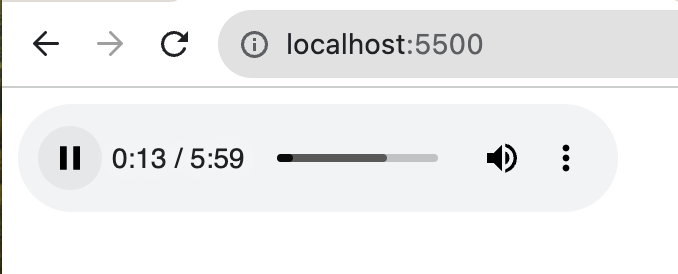
\includegraphics[trim=0cm 0cm 0cm 0cm, clip=true, width=0.75\textwidth]{img/audiobideo/audiocontrols.png}};
\end{tikzpicture}
\caption{Audio player-a, hainbat kontrolekin.}
\label{fig:audiocontrols}
\end{figure}


Nabigatzaileek audio-formatuekin duten bateragarritasun-maila jakin ahal izateko badugu Wikipedian orri berezi bat ere\footnote{\href{http://en.wikipedia.org/wiki/HTML5\_Audio}{http://en.wikipedia.org/wiki/HTML5\_Audio}}.

\section{Ariketak}

Ariketa multzo honetan canvas eta <video> etiketak uztartuko ditugu, adibidez \ref{fig:bideoariketa}. irudian dagoen ariketa egiteko. 

\begin{figure}[ht]
	\centering
\begin{tikzpicture}
\node[anchor=south west,inner sep=0] (image) at (0,0)
   {\includegraphics[trim=0cm 0cm 0cm 0cm, clip=true, width=0.75\textwidth]{img/azala.png}};
\end{tikzpicture}
\caption{Bideo batetik fotogramak atera daitezke eta canvas batean utzi baino lehen itxuraz aldatu. Adibidez, irudia zuri-beltz bihurtzeko.}
\label{fig:bideoariketa}
\end{figure}

Hemengo kode-adibideari jarraituz
\href{https://codesandbox.io/s/bideo-ariketa-1-bh3cg}{https://codesandbox.io/s/bideo-ariketa-1-bh3cg}:

\begin{enumerate}
    \item  Controls atributua ezabatu <video> etiketatik. Jarraian 3 botoi prestatu bideoaren azpian agertzeko: Jo, Eten, Kaptura.

\begin{itemize}
    \item Jo botoian sakatzean, bideoa martxan jarriko da.
     \item  Eten botoian sakatzean, bideoa eten egingo da. Berriro martxan jartzeko, Jo botoian sakatu.
     \item Kaptura botoian sakatzean, bideoaren uneko fotogramaren kaptura egingo da. Kaptura
     <canvas> etiketan bistaratu behar da, dimentsioak aldatuz —txikiagoa ikusi behar da bideoa baino, zuk aukeratu tamaina—. Adibide gisa, ikus \ref{fig:bideoariketa2}. irudia.
     
\begin{figure}[ht]
\centering
\begin{tikzpicture}
\node[anchor=south west,inner sep=0] (image) at (0,0)
   {\includegraphics[trim=0cm 0cm 0cm 0cm, clip=true, width=0.75\textwidth]{img/audiobideo/joetenkaptura.png}};
\end{tikzpicture}
\caption{Kaptura botoian sakatzean uneko fotogramaren kaptura egin behar da eta tamaina txikian margotu, irudian bezala.}
\label{fig:bideoariketa2}
\end{figure}
     
Argibidea:\textit{ drawImage()} metodoak lehenengo parametroan bideo baten erreferentzia onartzen du. 
\end{itemize}

Ariketaren soluzioa begiratu gabe egiten saia zaitez, baina argibideren bat behar baduzu, hona hemen ariketaren soluzioa:\newline \href{https://codesandbox.io/s/bideoariketak-soluzioa-i3kp8}{ https://codesandbox.io/s/bideoariketak-soluzioa-i3kp8}

\item Aurreko ariketa moldatu bideoaren kapturak automatikoki egin daitezen, alegia \textit{canvas} osagaian bideoaren fotogramak agertuko dira bideoa martxan dagoen bitartean, automatikoki.

Honako lerro hau lagungarria egingo zaizu:

\begin{lstlisting}[language=JavaScript,numbers=none]
bideoa.addEventListener("play", function () { .... zure kodea ... }
\end{lstlisting}

Bideoa amaitzen denean edo bideoa etetean (``pause'' egitean), \textit{canvas} osagaian fotogramak kopiatzeari utzi.

Beste lerro hau ere lagungarria egingo zaizu:

\begin{lstlisting}[language=JavaScript,numbers=none]
bideoa.addEventListener("pause", function () { ... zure kodea hemen ...}
\end{lstlisting}

Ariketaren soluzioa begiratu gabe egiten saia zaitez, baina argibideren bat behar baduzu, hona hemen: \href{https://codesandbox.io/s/bideosoluzioa2-jiqyn}{https://codesandbox.io/s/bideosoluzioa2-jiqyn}.


\item Hurrengo ariketan <video> eta <canvas> etiketak uztartuko ditugu. Helburua \ref{fig:bideoariketa}. irudian dugun aplikazio lortzea da. Goiko aldean bideo bat dugu. Haren azpian bi canvas txiki. Ezkerrekoan orain arte egin duguna.
Eskuinekoan zuri-beltzez margotuko dugun beste canvas bat. Prozesua honakoa da:

\begin{itemize}
    \item Bideotik frame bat atera eta ezkerreko canvas osagaian (\textit{buffer} deritzona) utzi:

buffer.drawImage(bideoa, 0, 0, 160, 120);

Jarraian, bufferetik frame baten informazioa erauzi, array gisa:

\begin{lstlisting}[language=JavaScript,numbers=none]
let frame = buffer.getImageData(0, 0, 320, 120);
\end{lstlisting}

frame arrayak \ref{fig:bideoariketa2}. irudiko itxura izango du:

\begin{figure}[ht]
\centering
\begin{tikzpicture}
\node[anchor=south west,inner sep=0] (image) at (0,0)
   {\includegraphics[trim=0cm 0cm 0cm 0cm, clip=true, width=0.75\textwidth]{img/audiobideo/rgba.png}};
\end{tikzpicture}
\caption{R = Red-Gorria, G = Green-Berdea, B = Blue-Urdina, A = Alpha-Gardentasuna.}
\label{fig:bideoariketa2}
\end{figure}
     

Alegia, pixel bakoitzak 4 balio izango ditu: R (\textit{red} edo kolore gorria), G (\textit{green} edo berdea), B (\textit{blue}
edo urdina), A (\textit{alpha} edo gardentasun-maila). Adibidez, pixel bat guztiz gorria eta  erdi gardena izango bagenu, orduan haren balioa (255, 0, 0, 100) izango litzateke. 

Zenbat pixel ditugun jakiteko, zatiketa sinple bat egin dezakegu:

\begin{lstlisting}[language=JavaScript,numbers=none]
let length = frame.data.length / 4;
\end{lstlisting}

Ondoren, pixel bakoitzeko, haren posizioa eta (r,g,b,a) balioak aterako ditugu eta horiekin
zuri-beltzez() izeneko funtzio bati deituko diogu, kolorez dagoen pixel bat zuri-beltz bihurtzeko:

\begin{lstlisting}[language=JavaScript,numbers=none]
for (let i = 0; i < length; i++) {
 let r = frame.data[i * 4 + 0];
 let g = frame.data[i * 4 + 1];
 let b = frame.data[i * 4 + 2];
 zuri-beltzez(i, r, g, b, frame.data);
 }
\end{lstlisting} 
 
 zuri-beltzez() funtzioa erraza da, kolore-osagai bakoitzaren balioak batu eta batezbestekoa lortuko
du hasieran (kolore grisa lortzeko). Ondoren pixel horri kolore grisa esleitzen dio:


\begin{lstlisting}[language=JavaScript,numbers=none]
function zuri-beltzez(pos, r, g, b, data) {
 var grisa = (r + g + b) / 3;
 data[pos * 4 + 0] = grisa;
 data[pos * 4 + 1] = grisa;
 data[pos * 4 + 2] = grisa;
}
\end{lstlisting}

Egitea falta zaigun bakarra zuri-beltzez lortu dugun frame arraya canvas-en margotzea da:
\begin{lstlisting}[numbers=none]
zuri-beltza.putImageData(frame, 0, 0);
\end{lstlisting}

Ariketaren soluzioa begiratu gabe egiten saia zaitez, baina argibideren bat behar baduzu, hona hemen: \href{https://juananpe.github.io/txuribeltz/}{https://juananpe.github.io/txuribeltz/}.

\end{itemize}

\item Audio-ariketa batekin jarraituko dugu. Hiru fitxategiz osatutako array bat dugularik:
\textit{[\textquotesingle{}audio1.mp3\textquotesingle{}, \textquotesingle{}audio2.mp3\textquotesingle{}, \textquotesingle{}audio3.mp3\textquotesingle{}]}, programa ezazu script bat hiru audio horiek jotzeko, bata bestearen atzetik. Bukatzean, lehenengoarekin jarraitu, amaigabeko begizta batean.

\item Web orri bat prestatu <audio> elementuarekin, baina \textit{controls} atributurik gabe (ez dira audio kontrolatzeko botoiak agertuko). Sortu 4 botoia: play, pause, bolumena igo eta bolumena jaisteko.
JavaScript erabili audioa jotzeko eta kontrolatzeko. Adibidez, erabiltzaileak play botoia sakatzean, audioa martxan jarri behar da (eta play botoia desgaitu behar da). Pause botoian sakatzean audioa eten egin behar da eta play botoia berriro gaitu. Argibidea: aztertu play(), pause() funtzioak, eta audio elementuaren volume atributuak.

\item Audio elementu batean hainbat source jarri daitezkela ikusi dugu. Horietatik nabigatzaileak bat aukeratuko du (onartzen duen lehenengo codec-a, adibidez). Baina nola jakin dezakegu zein izan den nabigatzaileak aukeratu duen audio mota? Argibidea: aztertu audio elementuaren loadeddata gertaera eta currentSrc atributua.

\item Fast Forward (FF) botoia gehitu. Botoia sakatzean audioaren uneko posizioa 10 segundu aurreratuko da.

\item Uneko posizioa bistaratzen duen geruza gehitu. Bertan uneko posizioa (minutu:segundu) eta audioaren iraupena uneoro bistaratu behar da. Argibidea: setInterval edo hobe, audioaren timeupdate gertaera kudeatuz lortuko duzu.

\end{enumerate}

%% 10. Biltegiratze lokala
\include{localstorage}
%% 11. Geokokapena
\include{geokokapena}
%% 12. Web Worker
\include{webworker}
%%% 13. Inprimakiak
\include{inprimakiak}
%% 14. WebSocketak
\include{websocket}
%%% 15. Service Worker APIa
\include{serviceworkers}
%%% 16. NodeJS
\include{nodejs}
%%% 17. Express
\chapter{ExpressJS}

Express edo ExpressJS \index{express} kode irekiko Node-rako web aplikazio dinamikoak programatzeko \textit{framework} bat da. Kapitulu honetan adibide batekin egingo dugu lan: bezeroen datuak kudeatzeko aplikazio sinple bat programatuko dugu, hasiera-hasieratik.

Bezeroen izen-abizenak eta helbidea elektronikoa gorde, editatu, ezabatu eta bistaratzeko inprimaki bat izango dugu. Lehendabiziko bertsioan datu horiek soilik memorian gordeko ditugu. Bigarren bertsioan, bezeroen datuak \textit{noSQL}\index{noSQL} motako datu-base batean gordeko ditugu (\textit{mongodb}\index{mongodb} izeneko datu-base batean, hain zuzen ere).

Has gaitezen, lehenengo eta behin, \textit{express} \textit{framework}-a instalatzen.

Lehenengo eta behin aplikazioa hasieratu beharko dugu, \hl{npm init} komandoaz.


\begin{lstlisting}[language=Bash,numbers=none]
$ npm init
Aplikazioaren izena: bezeroak
Bertsioa: 1.0
Deskribapena: bezeroen kudeaketa
Entry Point (nondik hasten den aplikazioa): app.js
Testak egiteko komandoa: momentuz hutsik
Git reepo: momentuz hutsik
keywords: hitz gakoak, momentuz hutsik
author: zure izena
lizentzia: momentuz hutsik

\end{lstlisting}

\textit{npm init} komandoa exekutatu ondoren, \textit{package.json} fitxategia sortuko da.

Jarraian, \textit{express} eta haren mendekotasun guztiak instalatuko ditugu:

\begin{lstlisting}[language=Bash,numbers=none]
$ npm install express --save
\end{lstlisting}

Bukatzeko, HTTP zerbitzari sinple bat programatuko dugu:

\begin{lstlisting}[language=JavaScript]
// app.js fitxategia

let express = require('express');
let path = require('path');

let app = express();
app.listen( 3000, function() {
	console.log("Zerbitzaria 3000 portuan entzuten");
})
\end{lstlisting}

Zerbitzaria martxan jartzeko, \hl{node app.js} komandoa landuko dugu.

Orain http://localhost:3000/ URLan sartzen bagara, erantzun bat jasoko dugu, baina ziur asko ez da guk espero dugun erantzuna izango:

\begin{lstlisting}[numbers=none]
"Cannot GET /"
\end{lstlisting}

Erroreak esan nahi du zerbitzariak ez dakiela nola erantzun bidali diogun GET\index{GET} motako eskaerari. Alegia, \textit{"/"} bidea (\textit{route})\index{route} ez dugula tratatu zerbitzarian.  GET motako bideak tratatzeko, metodo berri bat programatu behar dugu:

\begin{lstlisting}[language=JavaScript]
app.get("/", function(req, res) {
	res.send("Kaixo mundua!");
});
\end{lstlisting}

Orain bai, URL bera eskatzean (http://localhost:3000/), ``Kaixo mundua!'' mezua jasoko dugu erantzun gisa.

\begin{alertinfo}{Zer da \texttt{-{}-}save aukera?}
  \index{--save}\texttt{-{}-}save aukerarekin instalatu nahi dugun paketea package.json fitxategian mendekotasun gisa idatzi nahi dugula zehazten dugu. \texttt{-{}-}save aukera erabili ezean, mendekotasun-paketea gure ordenagailuan instalatuko da, baina ez dugu horren berri izango package.json fitxategian (alegia, beste garatzaileek ez dute jakingo mendekotasun hau gure aplikaziorako beharrezkoa dela).
\end{alertinfo}

\section{Baliabide estatikoak}

\index{app.get()}\textit{app.get()} edo \index{app.post()} \textit{app.post()} erabili behar dugu edozein HTML orria zerbitzatzeko? Ezin dugu HTML5en egindako orri estatiko bat zerbitzatu beste modu egokiago batean? Noski, horretarako \textit{express} aplikazioaren bideraketak zehaztu baino lehen (app.get, app.post zehaztu baino lehen) baliabide estatikoen karpeta non dagoen adierazi beharko dugu (kasu honetan, \textit{public} izeneko karpeta):

\begin{lstlisting}
app.use(express.static('public'))
\end{lstlisting}

\index{app.use}\textit{app.use} egiturari \index{middleware}\textit{middleware} deitzen zaio. Bideraketak baino lehenago egin behar diren beste ataza eta prozesuak zehaztuko ditugu middleware funtzioekin. Hurrengo ataletan gehiago sakonduko dugu middleware honetan, baina momentuz horrela utziko dugu.

Adibide gisa, \textit{public} karpetan orri estatiko hau utziko dugu, inprimaki sinple batekin, \textit{post.html} izenarekin:

\begin{lstlisting}

<!DOCTYPE html>
<html lang="en">
<head>
	<meta charset="UTF-8">
	<title>POST metodoa erabiltzen duen inprimakia</title>
</head>
<body>
<form action="/bezeroa" method="POST">
Izena: <input type="text" name="izena"><input type="submit" value="Bidali">
</form>
</body>
</html>
\end{lstlisting}

Nabigatzailean orri hori atzitzeko hurrengo URLa idatziko dugu:

\hl{http://localhost:3000/post.html}

Ohart zaitez URLan ez dugula \hl{public/post.html} idatzi. \textit{Express}-ek badaki besterik ezean, HTML orriaren fitxategi estatikoak public/ karpetan egon behar duela.

\section{GET parametroak URLan bidaltzen}

Nola bidali ahal diogu gure \textit{express} aplikazioari GET parametro bat? Alegia, demagun horrelako URL bat idatzita: http://localhost:3000/bezeroa/Oihane zerbitzariak eskaera jaso eta ``Kaixo Oihane'' mezuarekin erantzun behar duela (ikus \ref{fig:urlparametroak}. irudia). URLan agertzen den izena jasotzeko \textit{req.params}\index{req.params} objektua erabiliko dugu, honela:

\begin{lstlisting}
app.get('/bezeroa/:izena', function(req, res) {
  res.send("Bezeroaren izena: " + req.params.izena);
});
\end{lstlisting}

\begin{figure}[ht]
	\centering
\begin{tikzpicture}[framed]
\node[anchor=south west,inner sep=0] (image) at (0,0)
   {\includegraphics[trim=0cm 0cm 0cm 0cm, clip=true, width=0.75\textwidth]{img/urlparametroak.png}};
\end{tikzpicture}
\caption{URL batean bidaltzen diren parametroak (\textit{URL parameters}) jaso eta tratatu ahal dira \textit{req.params} erabiliz.}
\label{fig:urlparametroak}
\end{figure}


\section{GET parametroak eskaeran bidaltzen}
GET metodoan parametroak URLan bi modutara bidal daitezke: URL bidearen parte izanik (ikusi dugun bezala) edo URLaren azken zatian, eskaera (\textit{query string}\index{query string}) izeneko parametroetan, galdera-ikur baten ostean, honela:\newline
\href{http://localhost:3000/bezeroa/?izena=Oihane}{http://localhost:3000/bezeroa/?izena=Oihane}.

Eskaera-parametro horiek jasotzeko, \textit{req.params}\index{req.params} erabili ordez, \textit{req.query}\index{req.query} erabiliko dugu. Adibidez:

\begin{lstlisting}
app.get('/bezeroa', function(req, res) {
  res.send("Bezeroaren izena: " + req.query.izena);
});
\end{lstlisting}

Parametro bat baino gehiago bidali nahi izanez gero, aldagaiak \hl{\&} karaktereaz banatuko ditugu, honela: \href{http://localhost:3000/bezeroa/?izena=Oihane\&abizena=Pereira}{http://localhost:3000/bezeroa/?izena=Oihane\&abizena=Pereira}.

\begin{lstlisting}
app.get('/bezeroa', function(req, res) {
  res.send("Bezeroaren izena: " + req.query.izena);
  res.send("Bezeroaren abizena: " + req.query.abizena);
});
\end{lstlisting}

\section{POST parametroak}\index{POST}

Inprimaki baten datuak orokorrean POST bidez bidaltzen dira, ez GET bidez. Nola jaso POST balio horiek zerbitzarian? Eskaera (\textit{request}) baten \textit{body} atributuan daude parametro hauek. Adibidez, \index{req.body}\textit{req.body.izena}. Baina, besterik gabe, hau inplementatzen badugu:

\begin{lstlisting}
app.post('/bezeroa', function(req, res) {
    res.send("Bezeroaren izena:" + req.body.izena;
}
\end{lstlisting}

ez dugu ezer jasoko. Zergatik? Arazoa da POST parametroak bide edo \textit{route} batean sartu baino lehen tratatu egin behar direla. Nabigatzaileak bidaltzen dituen datuak zerbitzarian jaso eta bideratu baino lehen tratatu egin nahi baditugu, \textit{express}-en middleware izeneko funtzioak erabili beharko ditugu.

Middleware bat erabiltzeko, aurreko gaian ikusi dugunez, \textit{app.use(funtzioa)} erabiliko dugu, bideraketak egin baino lehen. Kasu honetan, \index{body.parser}\textit{body.parser} izeneko middlewarea erabili genezake POST bidez datozen parametroak tratatzeko. Hala ere, ez da beharrezkoa izango, Express 4.16 bertsiotik aurrera, \index{body.parser}\textit{body.parser} middleware hau jada integratuta dago.
Beraz, nahikoa da ondorengoa egitea:

\begin{lstlisting}[language=JavaScript]
// application/x-www-form-urlencoded
app.use(express.urlencoded({ extended: true }))
\end{lstlisting}

Horrekin aurreko kodeak ondo funtzionatuko du. 

\begin{lstlisting}[language=JavaScript]
// parseatu  application/x-www-form-urlencoded datuak
app.use(express.urlencoded({ extended: true }))
app.post('/bezeroa', function(req, res) {
    res.send("Bezeroaren izena:" + req.body.izena;
}
\end{lstlisting}

\begin{alertinfo}{x-www-form-urlencoded}
\ref{fig:form-urlencoded}. irudian ikusten dugunez, form baten datuak POST bidez bidaltzean, besterik ezean, HTTP eskaeraren eduki mota (Content-Type) application/x-www-form-urlencoded izango da.
\end{alertinfo}





% \begin{figure}[ht]
% 	\centering
% \begin{minipage}{.4\textwidth}
% \begin{tikzpicture}[scale=0.5]
% \node[anchor=south west,inner sep=0] (image) at (0,0)
%    {\includegraphics[trim=0cm 0cm 0cm 0cm, clip=true, width=1.0\textwidth]{img/form-urlencoded.png}};
% \end{tikzpicture} % pic 1
% \end{minipage}
% \begin{minipage}{.4\textwidth}
% \begin{tikzpicture}[scale=0.5]
% \node[anchor=south west,inner sep=0] (image) at (0,0)
%    {\includegraphics[trim=0cm 0cm 0cm 0cm, clip=true, width=1.0\textwidth]{img/urlparametroak.png}};
% \end{tikzpicture} % pic 2
% \end{minipage}
% \caption{xxxx}
% \label{fig:form-urlencoded}
% \end{figure}

\begin{figure}[ht]
	\centering
\begin{tikzpicture}[framed]
\node[anchor=south west,inner sep=0] (image) at (0,0)
   {\includegraphics[trim=0cm 0cm 0cm 0cm, clip=true, width=0.75\textwidth]{img/form-urlencoded.png}};
\end{tikzpicture}
\caption{Form baten datuak bidaltzeko bi metodo daude: POST eta GET. GET kasuan, datuak URLan ikusiko dira. POST kasuan, HTTP eskaeraren edukian joango dira eta eskaeraren eduki mota \textit{application/x-www-form-urlencoded} izango da.}
\label{fig:form-urlencoded}
\end{figure}

\section{Nodemon}\index{nodemon}
Orain arte \hl{index.js} edo beste edozein JS fitxategitan aldaketa bat egitean, \textit{express} zerbitzaria itzali eta berriro martxan jarri behar izan dugu, aldaketak har zitzan. Baina edizio-prozesu hori oso astuna bilaka daiteke. Hoberena izango litzateke modulu bat izatea JS fitxategietan aldaketak automatikoki antzematen dituena eta berak bakarrik zerbitzaria berrabiarazten duena. Hori da, hain zuzen ere, \hl{nodemon} izeneko tresnaren zeregina. nodemon instalatzeko npm erabiliko dugu:

\begin{lstlisting}
$ npm install -g nodemon    
\end{lstlisting}

-g parametroak instalazio globala egin nahi dugula adierazten du. Hortik aurrera, erabiltzaile guztiek eskuragarri izango dute nodemon aplikazioa, ez soilik uneko erabiltzaileak. Behin instalatuta erabili egingo dugu:

\begin{lstlisting}
$ nodemon index.js
\end{lstlisting}

Orain, edozein aldaketa egiten badugu \hl{index.js} fitxategian, \textit{nodemon}-ek automatikoki aldaketa antzeman eta zerbitzaria automatikoki berrabiaraziko du. 

\section{Txantiloiak: EJS}\index{ejs}
Web garapenean diharduten enpresetan web programatzaileak eta web diseinatzaileak izaten dituzte. Orokorrean, programatzaileek aplikazioaren kodea programatzen dute eta diseinatzaileek web orrien itxura moldatzen dute, alegia, orrien diseinu grafikoa. Diseinatzaileek orri baten txantiloia prestatzen dute gero programatzaileek aplikazioaren datuekin betetzeko (adibidez, datu-base batetik ekarritako datuekin). Express-ek ere HTML txantiloi baten gainean datuak bistaratzeko aukera ematen du. Izan ere, hainbat modulu daude txantiloiekin lan egiteko (\textit{ejs, pug, mustache, handlebars, jade}...). Liburu honetan ejs erabiliko dugu, erraza baita berarekin lan egitea.

Lehenengo eta behin, \textit{ejs} instalatu egin behar da:

\begin{lstlisting}
$ npm install ejs  --save
\end{lstlisting}

Jarraian, txantiloiak kudeatzeko ejs erabiliko dugula zehaztuko dugu (9. lerroan):

\begin{lstlisting}[language=JavaScript]
const express = require('express');
const path = require('path');
const bodyParser = require('body-parser')

const app = express();

app.use(express.static('public'))

app.set('view engine', 'ejs');
app.set('views', path.join(__dirname, 'views'));
\end{lstlisting}

10. lerroan txantiloiak zer karpetatan gordeko ditugun adierazten da (lerro horrek \textit{path} moduluarekin mendekotasun bat dauka, horregatik inportatu behar dugu 2. lerroan)

Orain, erro-katalogoa eskatzean, ez dugu zuzenean ``Kaixo mundua!'' katearekin erantzungo:

\begin{lstlisting}[language=JavaScript]
app.get("/", function(req, res) {
    res.send("Kaixo mundua!");
});
\end{lstlisting}

baizik eta, horren ordez, \hl{index.ejs} txantiloia bidaliko dugu:

\begin{lstlisting}
app.get("/", function(req, res) {
    res.render('index');
});
\end{lstlisting}

\hl{index.ejs} txantiloiaren edukian \ref{fig:ejs}. irudian daukagun kodea sartuko dugu, hots:

\begin{lstlisting}
<!doctype html>
<html lang="en">
<head>
    <meta charset="UTF-8">
    <title>EJS probatzen</title>
</head>
<body>
    Kaixo EJS txantiloi kudeatzailetik
</body>
</html>
\end{lstlisting}

\begin{figure}[ht]
	\centering
\begin{tikzpicture}[framed]
\node[anchor=south west,inner sep=0] (image) at (0,0)
   {\includegraphics[trim=0cm 0cm 0cm 0cm, clip=true, width=1.0\textwidth]{img/ejs.png}};
\end{tikzpicture}
\caption{EJS txantiloiak probatzeko, \hl{views/} izeneko karpeta bat sortu dugu eta bertan \hl{index.ejs} fitxategia sartu.}
\label{fig:ejs}
\end{figure}

Orain arte ikusi dugunaren arabera, ez dugu inolako aldaketarik somatzen EJS txantiloi baten eta HTML orri estatiko baten aldean (public/ karpetan ditugun orrien artean). Ezberdintasun nagusia da txantiloiek parametroak onartzen dituztela. Adibidez, \hl{app.get(\textquotesingle{}/\textquotesingle{})} kudeatzailetik parametro bat pasatu nahi badiogu txantiloiari, honakoa idatziko dugu \hl{index.ejs} fitxategiaren \textit{title} atalean, izenburua parametro gisa jasotzeko:

\begin{lstlisting}[language=HTML]
<title><%=izenburua %></title>    
\end{lstlisting}

Alegia, EJS aldagai bat \hl{<\% \%>} ikurren artean sartuko dugu. Eta aldagai hori txantiloian bistaratu nahi badugu, \hl{<\%=aldagaia\%> } idatziko dugu.

Bukatzeko, app.get(\textquotesingle{}/\textquotesingle{}) kudeatzailea honela geratuko da:

\begin{lstlisting}[language=JavaScript]
app.get("/", function(req, res) {
    res.render('index', {
        'izenburua': 'Kaixo EJS txantiloi kudeatzailetik'    
    }) 
});
\end{lstlisting}

Txantiloia ondo dabilela probatu baino lehen, \hl{public/} karpetatik \hl{index.html} ezabatu egingo dugu. Ez badugu egiten, \textit{express}-ek hor aurkituko du \textit{index} izeneko orri bat eta hori hobetsiko du txantiloiaren aurrean. 

Dena ondo badoa, \hl{http://localhost:3000} webgunea atzitzean, \ref{fig:txantiloia1-ejs}. irudian ikusten dugun emaitza lortu beharko genuke.

\begin{figure}[ht]
	\centering
\begin{tikzpicture}[framed]
\node[anchor=south west,inner sep=0] (image) at (0,0)
   {\includegraphics[trim=0cm 0cm 0cm 0cm, clip=true, width=.75\textwidth]{img/txantiloia-ejs.png}};
\end{tikzpicture}
\caption{EJS txantiloiek parametroak onartzen dituzte. Izenburuan ikus dezakegu orri honi pasatu diogun parametroa.}
\label{fig:txantiloia1-ejs}
\end{figure}

\subsection{Txantiloiak betetzen}

Demagun hiru bezeroren datuak ditugula:

\begin{lstlisting}[language=JavaScript]
let bezeroak = [
    {
        id: 1,
        izena: 'Ane',
        abizena: 'Uriarte',
        email: 'ane@ni.eus'
    },
    {
        id: 2,
        izena: 'Jon',
        abizena: 'Juanenea',
        email: 'jon@ni.eus'
    },
    {
        id: 3,
        izena: 'Oihane',
        abizena: 'Lete',
        email: 'oihane@ni.eus'
    },
]
\end{lstlisting}

Orain, datu horiek web orrian bistaratu nahi baditugu, parametro gisa pasa behar dizkiogu \hl{index.ejs} txantiloiari:

\begin{lstlisting}[language=JavaScript]
app.get("/", function(req, res) {
    res.render('index', {
        'izenburua': 'EJS probatzen',
        'bezeroak': bezeroak
    })
});
\end{lstlisting}

Eta index.ejs txantiloian datuak zeharkatu, \textit{forEach}\index{forEach} egitura erabiliz:

\begin{lstlisting}[language=HTML]
<!doctype html>
<html lang="en">
<head>
    <meta charset="UTF-8">
    <title><%=izenburua%></title>
</head>
<body>
    Kaixo EJS txantiloi kudeatzailetik
    <ul>
        <% bezeroak.forEach( function(bezeroa) { %>
        <li><%=bezeroa.izena %> <%=bezeroa.abizena%></li>
        <% }) %>
    </ul>
</body>
</html>
\end{lstlisting}

Dena ondo badoa, \hl{http://localhost:3000/} helbidean sartzean, \ref{fig:txantiloia-ejs}. irudiaren emaitza ikusiko dugu.

\begin{figure}[ht]
	\centering
\begin{tikzpicture}[framed]
\node[anchor=south west,inner sep=0] (image) at (0,0)
   {\includegraphics[trim=0cm 0cm 0cm 0cm, clip=true, width=.5\textwidth]{img/ejs-bezeroak.png}};
\end{tikzpicture}
\caption{Bezeroen datuak JSON array batean EJS txantiloiari ondo bidaltzen badizkiogu, honela ikusi beharko litzateke nabigatzailean.}
\label{fig:txantiloia-ejs}
\end{figure}

\section{Ariketa}
Prestatu inprimaki bat \hl{index.ejs} txantiloian, bezero berri baten datuak (izena, abizena eta helbide elektronikoa) zerbitzarira POST bidez bidaltzeko. Zerbitzariak datuak jaso eta pantailan bistaratuko ditu. 


%%% 18. testing
\chapter{Nola testatu Express aplikazioak}

Kapitulu honetan Express aplikazio bat testeatzen ikasiko dugu. Hemen proba unitarioak erabiliko ditugu soilik (proba funtzionalak, integrazio probak, erregresio probak etab. alde batera utziz). Eskarmentua baduzu Javaz landutako proba unitarioekin (\textit{JUnit framework}a erabiliz), bide luze bat jada aurreratu duzu: express-en egindako aplikazioak berdin testeatu daitezke, baina beste framework pare baten laguntzarekin: \index{Jest} eta \index{SuperTest}.

\begin{enumerate}

    \item Gauzak probatzen hasteko, express aplikazio sinple bat sortuko dugu:

\begin{lstlisting}[language=JavaScript,numbers=none]
$ express --view=ejs express-test
$ cd express-test
$ npm install    
\end{lstlisting}

\item 
    jest, supertest eta cross-env paketeak instalatu

(-D aukerak devDependencies - alegia, garatze-garaiko mendekotasunak- instalatzen ditu. Pakete horiek ez dira beharrezkoak aplikazioa martxan jartzeko edota erabiltzeko, soilik testeatzeko/garatzeko erabiliko ditugu)

\begin{lstlisting}[language=JavaScript,numbers=none]
$ npm install  -D jest supertest
$ npm install -g cross-env
\end{lstlisting}

\item 
package.json fixategian hau txertatu (node aplikazioak testeatu nahi ditugula esaten ari gara hemen, eta node\_modules karpetaren barruan dagoena ez dugula testeatu nahi)

\begin{lstlisting}[language=JavaScript,numbers=none]
....
"jest": {
 "testEnvironment": "node",
 "coveragePathIgnorePatterns": [
   "/node_modules/"
 ] 
 }...
\end{lstlisting}

Gutxi gora-behera horrelako package.json bat lortuko duzu:


\begin{figure}[ht]
	\centering
\begin{tikzpicture}
\node[anchor=south west,inner sep=0] (image) at (0,0)
   {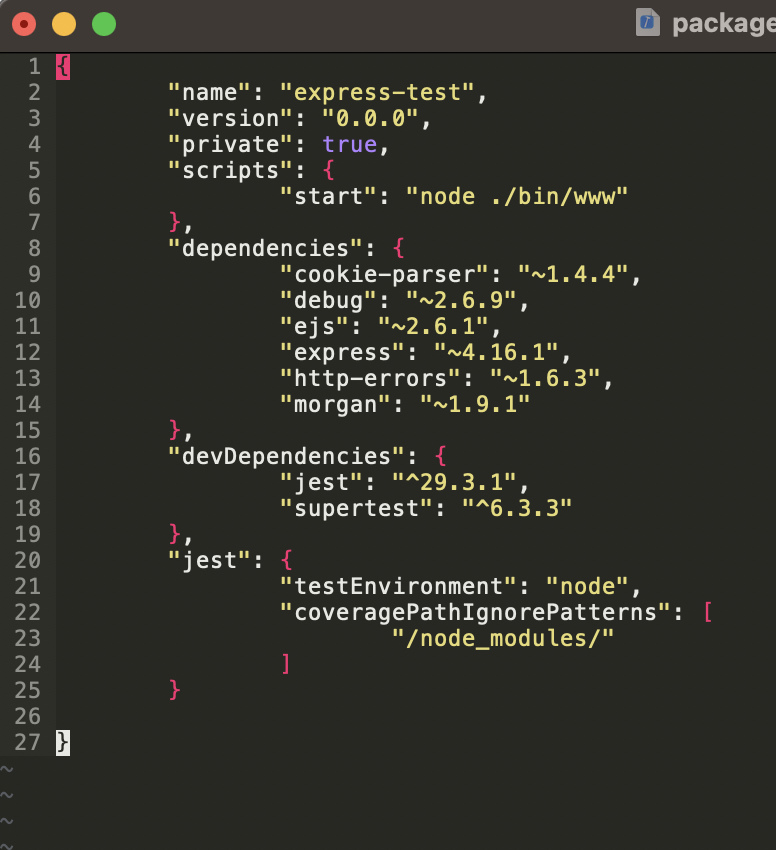
\includegraphics[trim=0cm 0cm 0cm 0cm, clip=true, width=0.75\textwidth]{img/testing/testing_package_json.png}};
\end{tikzpicture}
\caption{Testing: package json.}
\label{fig:testing-package-json}
\end{figure}


\item 
Jarraian, routes/users.js ezabatu eta routes/index.js fitxategiaren edukia Gist honen edukiarekin ordezkatu:

\href{https://gist.github.com/juananpe/8aa0cd571f07df8f278015ec476d3ecf}{https://gist.github.com/juananpe/8aa0cd571f07df8f278015ec476d3ecf}


Bertan, horrelako objektuak gorde (send), aldatu (update) eta ezabatzeko (destroy) rutak prestatu ditugu:

\begin{lstlisting}[language=JavaScript,numbers=none]
    const fakeDB = [
 {
   id: Math.floor(Math.random() * 100),
   email: "test@example.com",
 },
];
\end{lstlisting}

\begin{itemize}
    \item 

Oharra: adibidea errazteko, fakeDB objektua sortu dugu, mongoDB datubase bat simulatzen duena, array baten bidez.
\item 
Oharra: bi lerro hauek ezabatu app.js fitxategitik: 

\begin{lstlisting}[language=JavaScript,numbers=none]
var usersRouter = require('./routes/users');
....
app.use('/users', usersRouter);
\end{lstlisting}


\end{itemize}

\item 
package.json fitxategian, scripts atala horrela moldatu:


\begin{verbatim}
    
 "scripts": {
   "start": "node ./bin/www",
   "test": "cross-env NODE_ENV=test jest"
 },

\end{verbatim}


Oharra: NODE\_ENV bidez testeatzeko ingurune batean ari garela zehazten ari gara. Besteak beste 404 erroreak baldin badaude eta test ingurunean bagaude, orduan errorearen zergatia bistaratzen duen traza bat agertuko zaigu (traza horiek ez dira agertu behar production ingurunean, segurtasunaren aldetik informazio gehiegi - eta pribatua- ematen dutelako)


\item 
Aplikazioa martxan jarri:

\begin{verbatim}
cross-env PORT=4444 DEBUG="express-test:*" nodemon start    
\end{verbatim}


eta probatu ondo dabilela (eskuz, testak oraindik ez ditugu prestatu eta)

Zehazki, http://localhost:4444/ bidean, erantzun hau jaso beharko genuke:


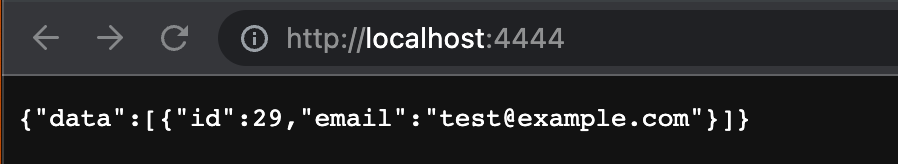
\includegraphics[width=0.75\textwidth]{img/testing/testing_view_index.png}

Berriz, POST \textbf{/send} endpoint-era eginez gero:

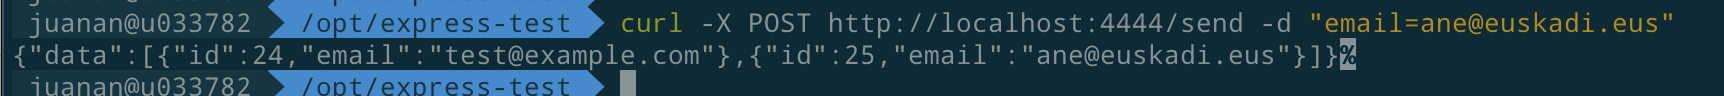
\includegraphics[width=0.75\textwidth]{img/testing/testing_post.png}

PUT endpoint-a probatzeko:

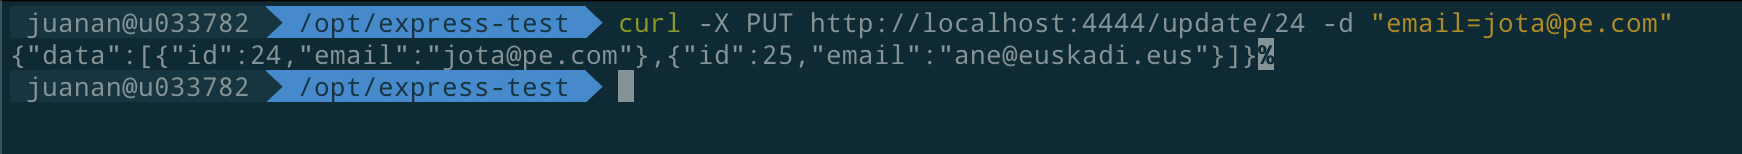
\includegraphics[width=0.75\textwidth]{img/testing/testing_put.png}


eta DELETE endpoint-a probatzeko:


\includegraphics[width=0.75\textwidth]{img/testing/testing_delete.png}

\item 
Dena ondo doala probatu ostean, zerbitzaria eten eta berriro martxan jarri

\item 
Sortu \textbf{tests} karpeta eta bertan fitxategi hau:

\begin{lstlisting}[language=JavaScript,numbers=none]
    /* server.test.js */

const request = require('supertest');
const PORT = process.env.PORT || 4444;
const url = `http://localhost:${PORT}`


describe('Testing index', () => {
   it('GET /', async () => {
       const res = await request(url).get('/');
       expect(res.statusCode).toBe(200);
       expect(res.type).toBe('application/json');
       expect(res.type).toMatch(/json/);
   });
   // hurrengo it()
});

\end{lstlisting}


\textbf{Azalpena:}

\begin{enumerate}
    \item lehenengo 3 lerroetan supertest paketea inportatu ondoren, gure aplikazioarekin lotzen dugu. 
\item jarraian describe() funtzioak test multzo (test suite) bat deskribatzen du. describe baten barruan hainbat it() (test) funtzio izan ditzakegu. Baina momentzu ez dugu ezer probatu. Berez, jarraian datozen funtzioekin egingo ditugu testak.
\item get('/') funtzioak GET request bat egingo du / bidera. Erantzuna res (response) objektuan dator. 
\item behin res (erantzuna) dugula, barruan dagoen objektuen atributuak espero ditugun balioen kontra konparatuko ditugu expect() funtzioekin. Adibidez, GET / egin ondoren HTTP status code = 200 izatea espero dugu (gogoratu HTTP/200 = OK)
\item toBe(), toMatch, etab. expect() objektuaren metodoak dira. Gainontzeko metodo guztiak ezagutzeko, botaiozu begirada bat URL honi: https://jestjs.io/docs/expect 

\end{enumerate}


\item 
Exekutatu testak 
(Oharra: jest komandoak *.test.js bilatu eta exekutatuko ditu, automatikoki)
\begin{verbatim}
$ npm test    
\end{verbatim}

Dena ondo badoa, hau ikusiko duzu:

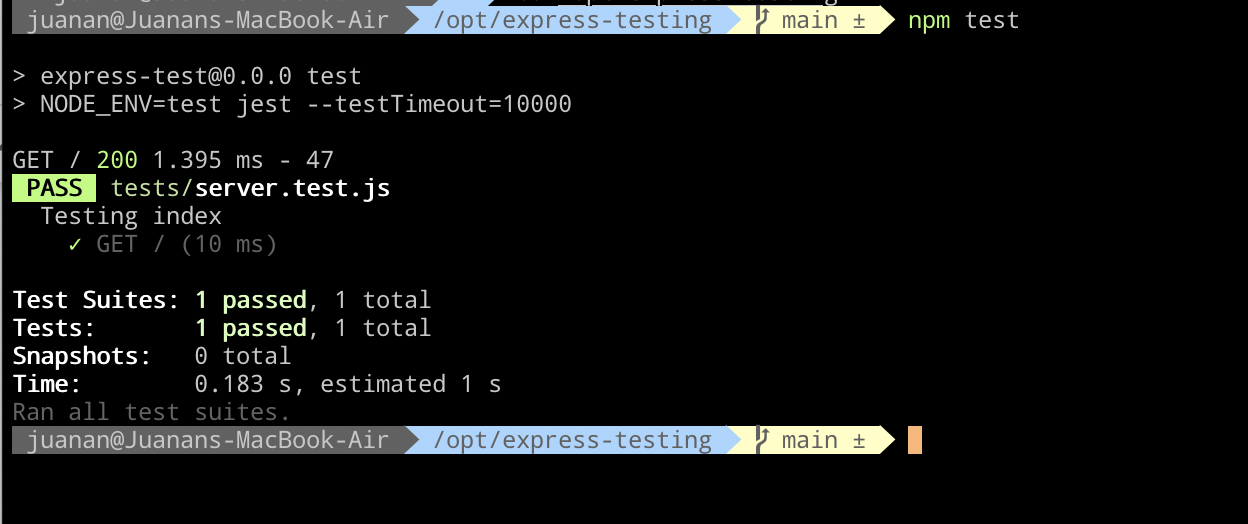
\includegraphics[width=0.75\textwidth]{img/testing/testing_npm_test.png}

\item 
Aurreko kode zatian, "//hurrengo it()" komentarioaren ondoren, hau sartu:

\begin{lstlisting}[language=JavaScript,numbers=none]
    it("POST /send", async () => {
   const res = await request(url).post("/send")
       .send({
           email: 'janire@example.com'
       });


   expect(res.type).toMatch(/json/)
   expect(res.statusCode).toBe(201)
   expect(res.body.data.length).toBe(2)
   expect(res.body.data[0].email).toMatch("test@example.com")
   expect(res.body.data[1].email).toMatch("janire@example.com")
})
\end{lstlisting}


Eta exekutatu berriro test multzoa, horrela:
\begin{verbatim}
$ npm test    
\end{verbatim}

Dena ondo badoa hurrengoa jaso beharko zenuke:

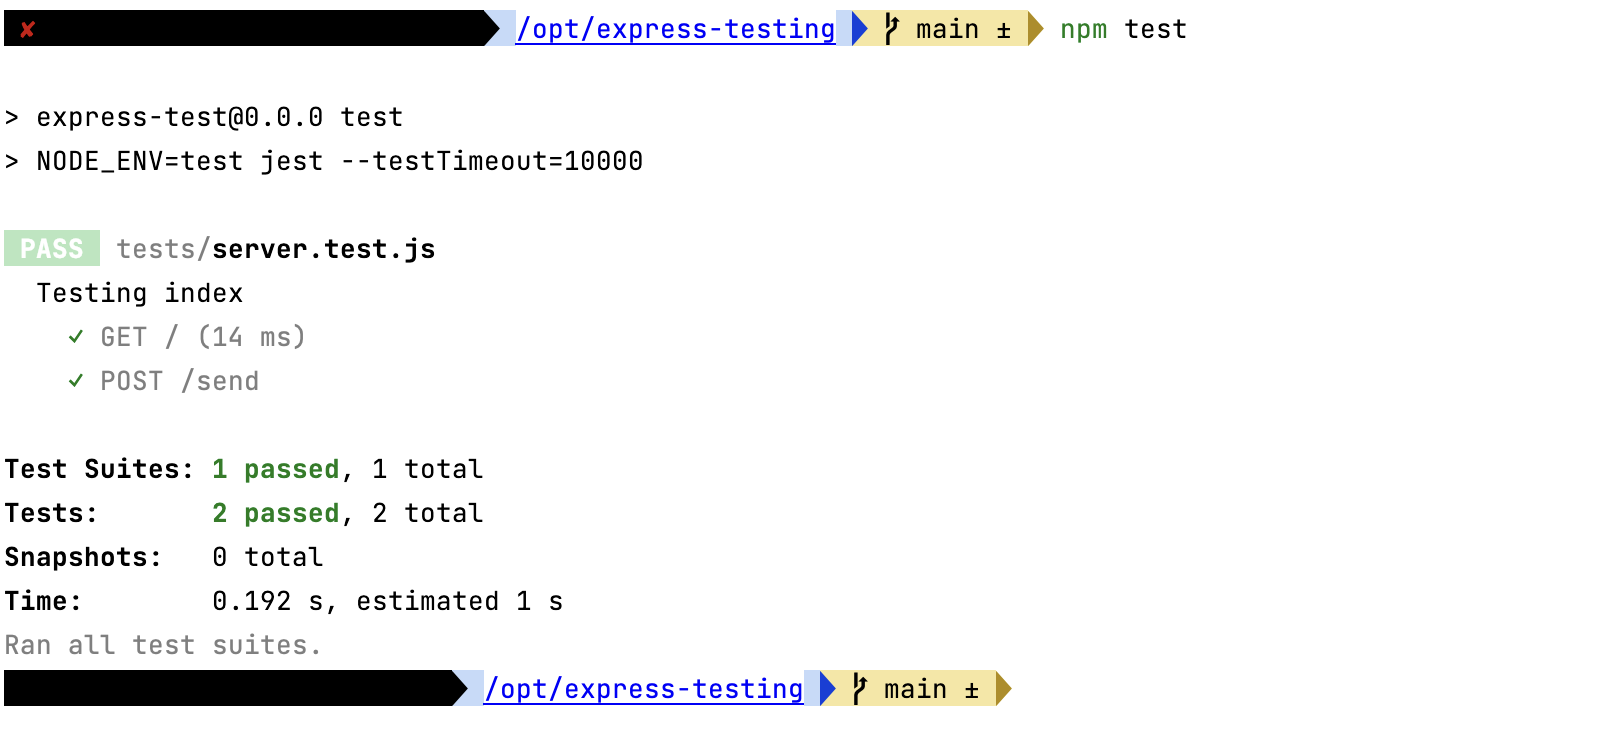
\includegraphics[width=0.75\textwidth]{img/testing/testing_npm_test_results.png}

\begin{itemize}
    \item 

Zer gertatuko litzateke janire@example.com ordez, maitane@example.com esperoko bagenu?

\begin{lstlisting}[language=JavaScript,numbers=none]
expect(res.body.data[1].email).toMatch("maitane@example.com")
\end{lstlisting}

Zein da jest exekutatzearen emaitza kasu honetan? (pantaila kaptura bat atera)

\end{itemize}

\item 
Orain beste erabiltzaile berri bat sartuko dugu, curl erabiliz:

\begin{lstlisting}[language=JavaScript,numbers=none]       
 curl -X POST http://localhost:4444/send/ -d "email=jota@gmail.com"

\end{lstlisting}


Ariketa: Nola aldatuko zenuke 10. ariketan egin dugun post() test-a 11. ariketan sartu dugun elementua ondo txertatu dela probatzeko?

\item 
Jarraian DELETE ruta probatuko dugu

Demagun hau dela uneko egoera:

\begin{verbatim}
  {"data":
    [{"id":52,"email":"test@example.com"}, 
     {"id":86,"email":"janire@example.com"},
      {"id":28,"email":"jota@gmail.com"}]}   


\end{verbatim}

Eta id:28-a duen elementua ezabatu nahi dugula. Lehenengo curl comandoaz probatuko dugu:

\begin{lstlisting}[language=JavaScript,numbers=none]
$ curl -X DELETE http://localhost:4444/destroy/28
{"data":    [{"id":52,"email":"test@example.com"},       {"id":86,"email":"janire@example.com"} ]
\end{lstlisting}

Ondo doala dirudi. 

Orain test bat prestatuko dugu. Horretarako, azken ID-a zein den kalkulatu ondoren (get() metodoaz) delete() bat exekutatuko dugu ID horren gainean)

\begin{lstlisting}[language=JavaScript,numbers=none]
it("DELETE /destroy/:id", async () => {
   const res = await request(url).get('/');
   const luzera = res.body.data.length
   // orduan azken elementua luzera -1 posizioan egongo da
   const id = res.body.data[luzera - 1].id
...
\end{lstlisting}

Jarraian id hori duen objektuaren ezabaketa ondo dabilela testeatuko dugu:

\begin{lstlisting}[language=JavaScript,numbers=none]
it("DELETE /destroy/:id", async () => {
   const res = await request(url).get('/');
   const luzera = res.body.data.length
   // orduan azken elementua luzera -1 posizioan egongo da
   const id = res.body.data[luzera - 1].id


   const response = await request(url).delete(`/destroy/${id}`);
   expect(response.type).toMatch(/json/)
   expect(res.statusCode).toBe(200);
   expect(response.body.data.length).toBe(luzera - 1)


})
\end{lstlisting}

Probatzeko:
\begin{verbatim}
$ npm test
\end{verbatim}

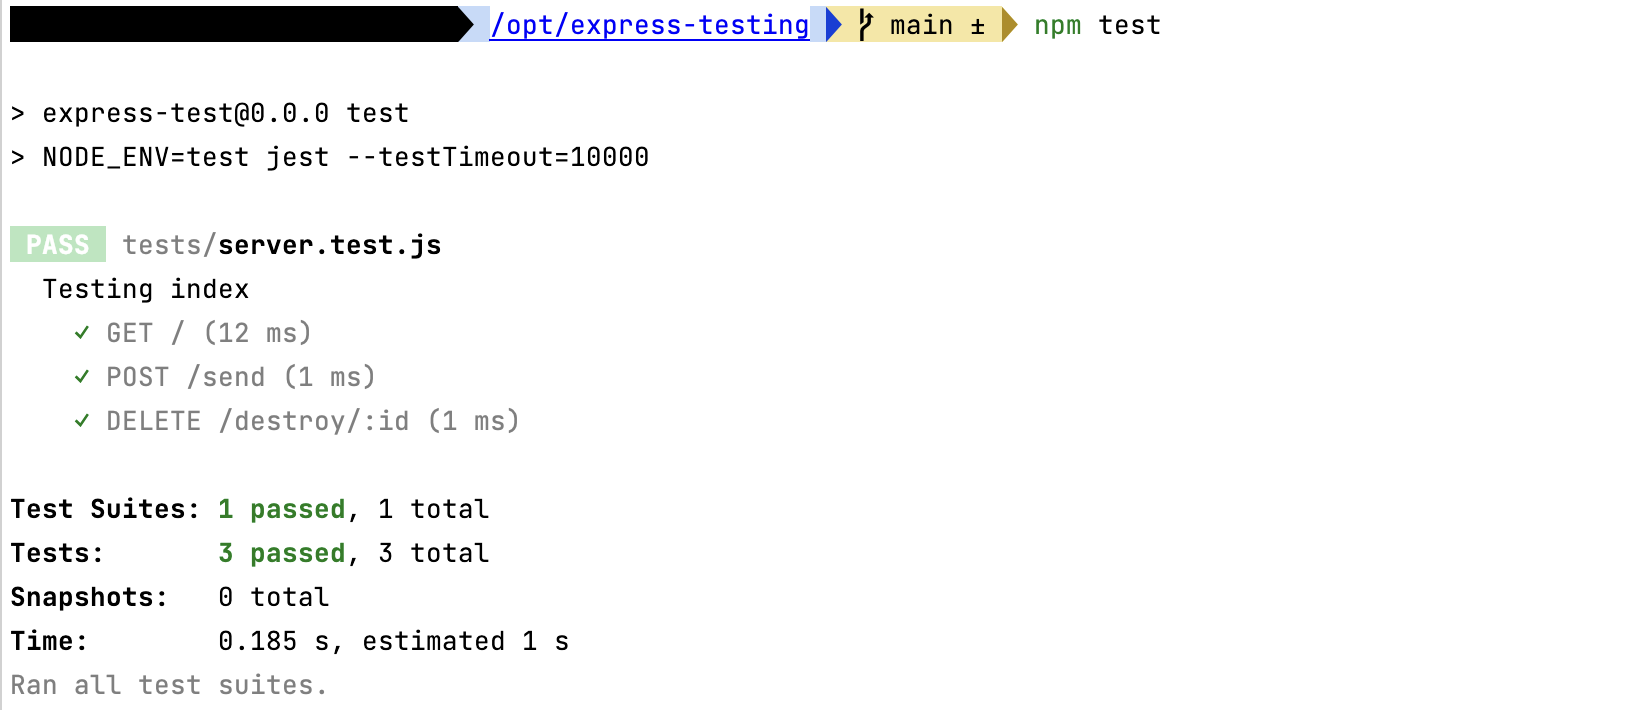
\includegraphics[width=0.75\textwidth]{img/testing/testing_npm_delete.png}

\item 
Ariketa: PUT ruta probatu

\begin{verbatim}
router.put("/update/:id", ....)    
\end{verbatim}


Horretarako:

\begin{itemize}
    \item 	13.1) Zein da CURL aplikazioaz probatzeko komandoa?
	(demagun lehenengo elementuaren email-a aldatu nahi dugula, test@example.com izan ordez, erabiltzaile@example.com izan dadila)

Erabili CURL aplikazioa lehenengo elementuaren emaila berriro test@example.com izan dadin.

\item 
13.2) Programatu test bat Jest eta SuperTest erabiliz (oinarritu zaitez 12. ariketan, oso-oso antzekoak baitira)

\end{itemize}
\end{enumerate}




%%% 19. mongodb 
\include{mongodb}
%%% 20. Firefoxen Web Kontsola
\include{araztailea}
%%% 21. IntelliJ eta VSCode
\include{IDEak}

% https://tex.stackexchange.com/questions/446839/makeidx-printindex-problem-is-there-one-way-to-redefine-index-name-as-chapter
% \stepcounter{chapter}
\phantomsection
\printindex

\end{document}
